%*******************************************************************************
% Master TeX file for 6x9 books
% Copyright A K Peters, Ltd.
%
% This is the main TeX file that is to be compiled.
%*******************************************************************************
\documentclass{book}

%*******************************************************************************
% Layout
%
% This defines the size of the page, etc. DO NOT EDIT.
%*******************************************************************************
\usepackage{geometry}

\geometry{
  paperwidth=6in,
  paperheight=9in,
  width=27pc,
  height=45pc, % textheight + head + headsep = 45pc
  headsep=12pt,
  foot=24pt,
  inner=0.9375in, % 15/16 in. gutter margin
  top=0.625in, % head margin
  includehead
}

% draws crop marks
\usepackage[cam,center,letter,noinfo]{crop}

\newcommand*\altcropulc{%
\begin{picture}(0,0)
 \unitlength = 1pt
 \thinlines
 \put(-30,0){\circle{10}}
 \put(-30,-5){\line(0,1){10}}
 \put(-35,0){\line(1,0){21}}
 \put(0,30){\circle{10}}
 \put(-5,30){\line(1,0){10}}
 \put(0,35){\line(0,-1){21}}
 \end{picture}
}

\newcommand*\altcropurc{%
 \begin{picture}(0,0)
 \unitlength = 1pt
 \thinlines
 \put(30,0){\circle{10}}
 \put(30,-5){\line(0,1){10}}
 \put(35,0){\line(-1,0){21}}
 \put(0,30){\circle{10}}
 \put(-5,30){\line(1,0){10}}
 \put(0,35){\line(0,-1){21}}
 \end{picture}%
}

\newcommand*\altcropllc{%
 \begin{picture}(0,0)
 \unitlength = 1pt
 \thinlines
 \put(-30,0){\circle{10}}
 \put(-30,-5){\line(0,1){10}}
 \put(-35,0){\line(1,0){21}}
 \put(0,-30){\circle{10}}
 \put(-5,-30){\line(1,0){10}}
 \put(0,-35){\line(0,1){21}}
 \end{picture}%
}

\newcommand*\altcroplrc{%
 \begin{picture}(0,0)
 \unitlength = 1pt
 \thinlines
 \put(30,0){\circle{10}}
 \put(30,-5){\line(0,1){10}}
 \put(35,0){\line(-1,0){21}}
 \put(0,-30){\circle{10}}
 \put(-5,-30){\line(1,0){10}}
 \put(0,-35){\line(0,1){21}}
 \end{picture}%
 }

\cropdef\altcropulc\altcropurc\altcropllc\altcroplrc{altcrop}

\crop[altcrop]

%*******************************************************************************
% Style file
%*******************************************************************************
\usepackage{akpbook}

%*******************************************************************************
% Packages
%
% Here you can add your own packages, if necessary, that are not covered by akpbook.sty
%*******************************************************************************
%---BEGIN AUTHOR EDIT---

\usepackage{placeins}
\usepackage{tabularx}
\usepackage{algorithmic}
\usepackage{algorithm2e}
\usepackage{multirow}


%---END AUTHOR EDIT---

%*******************************************************************************
% Declarations
%
% Any custom commands, aliases, or other declarations should be added to
% a separate TeX file, called [your last name]Macros.tex (e.g., SmithMacros.tex)
%*******************************************************************************
%---BEGIN AUTHOR EDIT---

%\include{[your last name]Macros}

%---END AUTHOR EDIT---

%*******************************************************************************
% Figure folders
%
%   Save you figures in a subfolder of the folder that contains this TeX file,
%   called Figures.
%
%   Uncomment the line below if your article contains figures.
%
%   Figures can then be included in the document using:
%
%   \includegraphics[width=\textwidth](FigFileName.eps}
%
%   or similar command.
%*******************************************************************************
\graphicspath{{Figures/}} % you may uncomment this line if needed

%*******************************************************************************
% Book
%*******************************************************************************
\makeindex
\begin{document}

\mainmatter
 \renewcommand{\chaptermark}[1]{\markboth{\thechapter. #1}{}}
 \renewcommand{\sectionmark}[1]{\markright{\thesection. #1}}

%*******************************************************************************
% Your Chapter
%
% The main body of your article should be a file called [your last name].tex.
%
% For the sake of this template, we provide a file called Smith.tex. You should
% edit the line below to match the name of your file, i.e., your last name.
%*******************************************************************************

%---BEGIN AUTHOR EDIT---
%*******************************************************************************
% Example chapter file for books
% Copyright A K Peters, Ltd.
%*******************************************************************************
\chapter{Real-Time Layered Materials Compositing Using Spatial Clustering Encoding}{Sergey Makeev}
 \label{Makeev-chapter}

\section{Introduction}

Most of the modern rendering engines take advantage of using a library of simple and well-known materials and a layered material representation to author detailed and high-quality ingame materials.
Popular tools used in texturing pipeline nowadays (e.g. "Allegorithmic Substance Painter" and "Quixel NDO Painter") are also based on the concept of layered materials
\cite{MaterialsOrder1886,TexturingU4,ShadingUE4}.

In this chapter, we present an algorithm that uses a layered materials method which allows us to create composite materials using a large number of layers in real-time.
Our algorithm is designed to mimic "Allegorithmic Substance" texture pipeline as close as possible but in real-time.
The proposed technique based on the blending of multiple well-known materials where a shared materials library defines the surface properties for each material used in compositing.

Using our method, each mesh can have one unique UV-set and several unique texture blend masks where each blend mask defines the per-pixel blending weights for the material from the library.
Each material from the library can use a detail textures technique to improve surface details resolution.
Using the materials with detail textures for the composition has the advantage of breaking the texture resolution barrier and allows us to produce a final composition at a very high resolution.
Having high-resolution in-game materials is especially crucial in the 4K era.

Our method supports the replacement of a library of materials and transparency modifications for the texture blend masks at runtime.
Material replacement at runtime leads to a different visual appearance of the resulting composited material which is especially important for games supporting User Generated Content or in-game Customization.
The presented technique is used for rendering armored vehicles in "Armored Warfare", an action multiplayer tank game published by My.com.

\section{Overview of Current Techniques}

A popular method for compositing is to pre-bake a multilayered material into a set of textures (albedo, normal, roughness, etc.) that are used by the game engine.
The resulting texture set are primarily designed for a specific mesh and cannot be shared between different meshes.
We call this method "Static Material Layering."
\cite{MaterialsOrder1886,TexturingU4}.
This approach gives good results but requires a lot of GPU memory to store the final high-resolution textures.


To break this limitation, some modern rendering engines use a technique that is pretty similar to the method that has already been proven for rendering terrain which is called "Texture Splatting."
\cite{TexSplatting}.
To produce the final composited texture, these engines blend several textures using a pixel shader and a set of texture blend masks which define the transparency of the blending.
We call this method "Dynamic Material Layering."
\cite{LayeredMaterialUE4,LayeredMaterialSubstance}.
This approach works well as shown in Figure~\ref{Makeev-DynamicMaterialLayering} but is limited to a small number of simultaneous material layers due to memory and performance limitations.

\begin{figure}\centering
\includegraphics[width=\textwidth]{SimpleLayersComp}
\caption{
An example of Dynamic Material Layering.
This example mesh uses three texture blend masks to define the blending transparency and three library materials to define the surface properties.
}
\label{Makeev-DynamicMaterialLayering}
\end{figure}

\section{Introduced Terms}

Since different game engines and material authoring pipelines use different terms, here are definitions which are used in this article.

\begin{itemize}  
\item \textbf{Material Template.}
One single well-known material such as gold, steel, wood, etc.
Material Template can use a tiled detail texture to give the illusion of greater detail for a material.
Material Templates are used as basic blocks to create complex multi-layered materials.
\item \textbf{Material Mask.}
A grayscale texture which is used for defining transparency while compositing different Material Templates. 
Usually these textures are created by modern texturing tools like "Allegorithmic Substance Painter" and "Quixel NDO Painter" using a semi-procedural approach.
\item \textbf{Color ID.}
A color-coded texture which defines areas of UVs that belong to different opaque materials.
The opaque material does not have a blend mask associated with it, and it is always used as a bottom layer in our composition.
A color-coded representation where each unique color represents a single material is used to simplify the content pipeline and reduce the number of required textures.
Each color-coded texture can represent several opaque materials as shown in Figure ~\ref{Makeev-ColorIds}.
\item \textbf{Layered Material.}
This is a material definition which is used to build the final composite material.
Each Layered Material has a single Color ID associated with it and an ordered set of Material Masks which define the composition order and the blending weights of the materials.
Layered Material also has a set of Material Templates associated with it to define the visual appearance of each material used in a composition.
\end{itemize}

\begin{figure}\centering
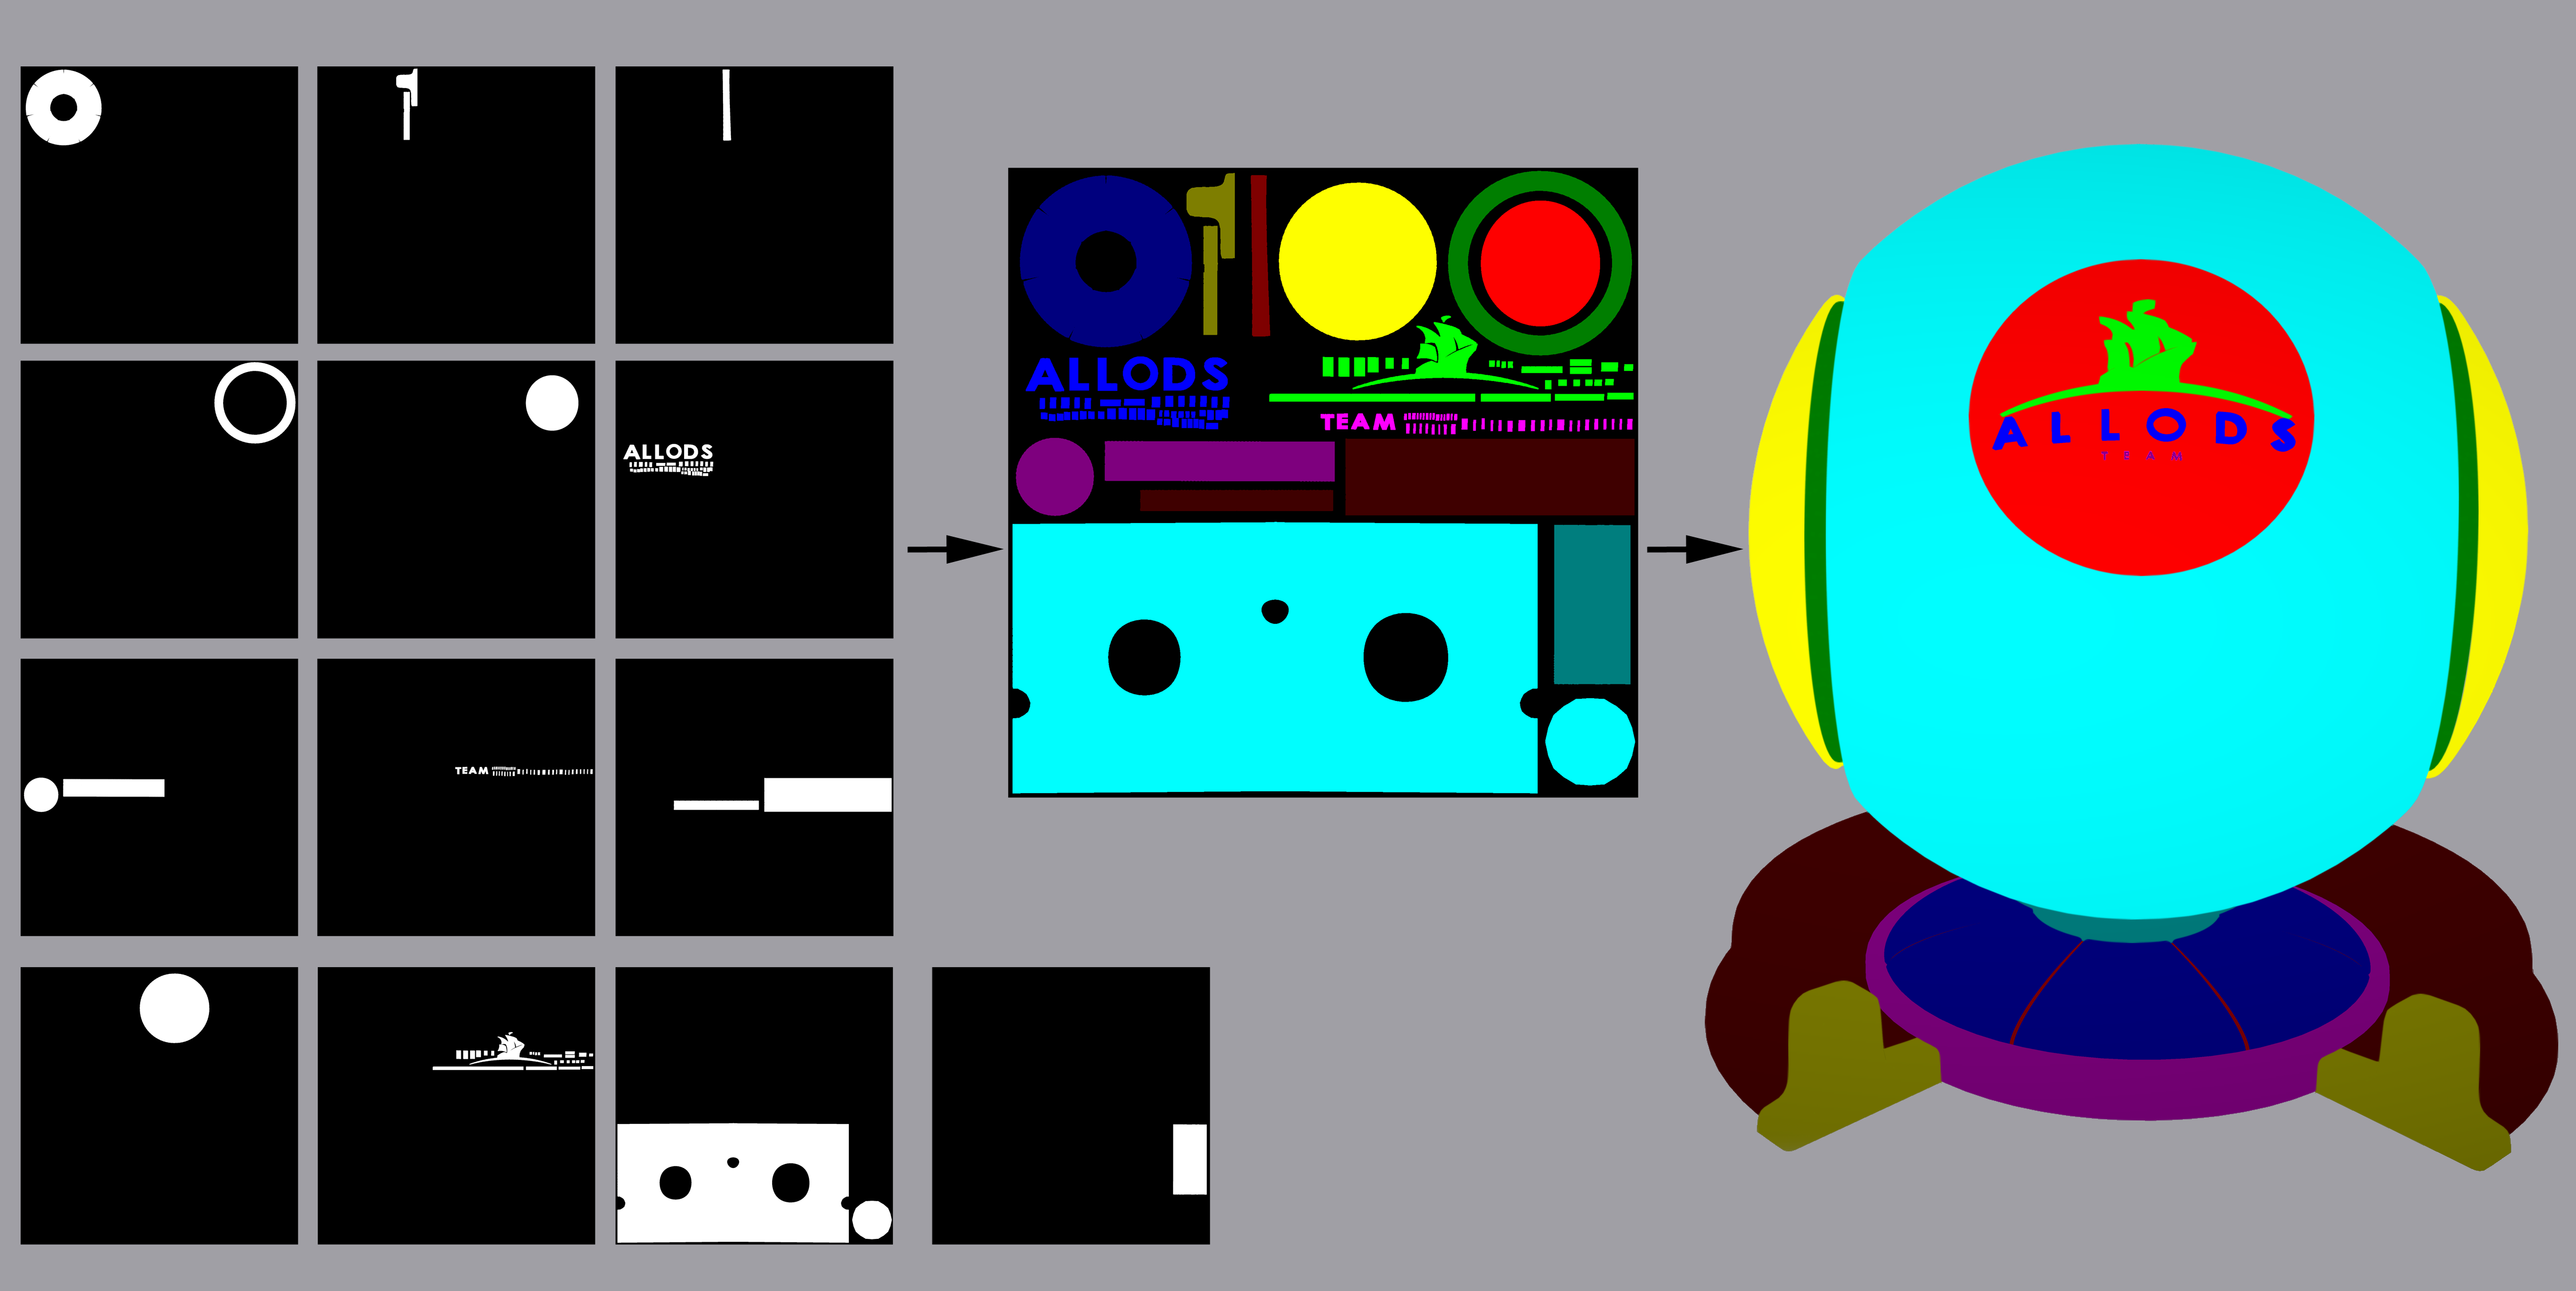
\includegraphics[width=\textwidth]{ColorIDs}
\caption{Several opaque material masks combined into a single Color ID map and applied to the mesh.}
\label{Makeev-ColorIds}
\end{figure}

\section{Algorithm Overview}

Existing solutions \cite{LayeredMaterialUE4,LayeredMaterialSubstance} which used for Dynamic Material Layering store transparency for different materials in RGBA channels of the texture.
When each material mask covers only a small area of the texture such solutions are inefficient in terms of memory consumption.
A lot of texture space is not used for the composition and wasted.


We observe that blend masks are usually coherent in the texture space and only partially overlap each other.
Using this observation, we propose storing the different non-overlapped blend masks in the same texture channels.
To achieve this, we group several Material Masks into a set that we call Clusters.
We build the clusters based on the connectivity between texels in texture space.
This allows us to use the texture space more effectively since the different clusters can store their blend masks in the same shared texture channels.
At runtime we use this clustered representation and the set of the material templates to make the final material composition as shown in Figure~\ref{Makeev-TechniqueExample}.


Since we are storing the different blend masks in the same texture channels, it is critical to take into account texture filtering boundaries between different clusters.
Texture filtering of different blend masks lead to errors during the composition stage due to the leaking of texture blend masks from one material into another.
While building the material clusters, we consider which neighboring pixels are involved in the texture filtering and this information is used while creating the clusters.

\begin{figure}\centering
\includegraphics[width=\textwidth]{allodsteam}
\caption{
An example of the use of the presented technique.
Several texture blend masks encoded as a single RGB weights texture and a single cluster indirection texture.
Encoded material blend masks and material templates from the library are composited to get the final image.
}
\label{Makeev-TechniqueExample}
\end{figure}

To create the initial partitioning into the clusters, we perform a connectivity analysis for the set of Material Masks.
Connectivity analysis classifies all the texels which are used for texture filtering as connected.
If the texels are classified as connected, they will belong to the same material cluster.
When we perform a connectivity analysis, we should also take mipmap texture filtering into account.
At the same time, we should limit the number of supported mipmap levels otherwise at the very last mipmap level all the texels will be classified as connected.
For our implementation, we decided to support only the first four mipmap levels.
Smaller mipmap levels are not handled by our implementation and discarded.
Supporting only the first four mipmap levels is enough to preserve a good quality of the texture filtering and keep the number of the resulting clusters small.
An incomplete mipmaps chain might lead to aliasing, but its level is acceptable \cite{VirtualTexturesMittring}.
In practice, the resulting aliasing can be barely visible and effectively removed by most of the modern anti-aliasing algorithms.


Each resulting cluster should not contain more than a limited number of materials where the number of materials depends on how many per pixel material layers we need to support.
In practice, the number of materials used in the cluster is usually equal to four or five since we store the cluster blend weights in the BC1 or BC3 texture format.
A practically unlimited total number of materials and five per-pixel materials is enough to represent even a very complex layered material.

Constructing the clusters with a limited number of materials is not always possible since we can find more connected materials than the maximum allowed number of materials per cluster.
As a result, we can find a cluster which is used more than a maximum allowed number of materials.
We can split such clusters into several smaller ones that meet our initial requirements.
This will lead to a texture filtering error for the texels shared between the clusters edges.
Filtering errors will occur due to erroneous texture filtering between blend masks from the different clusters in which different materials are encoded (see Figure~\ref{Makeev-MaskFilteringError}).
We propose a solution that minimizes leaking of the texture blend masks while splitting such clusters.
For more details see Section~\ref{Makeev-SolveGraphPartition}.

\begin{figure}\centering
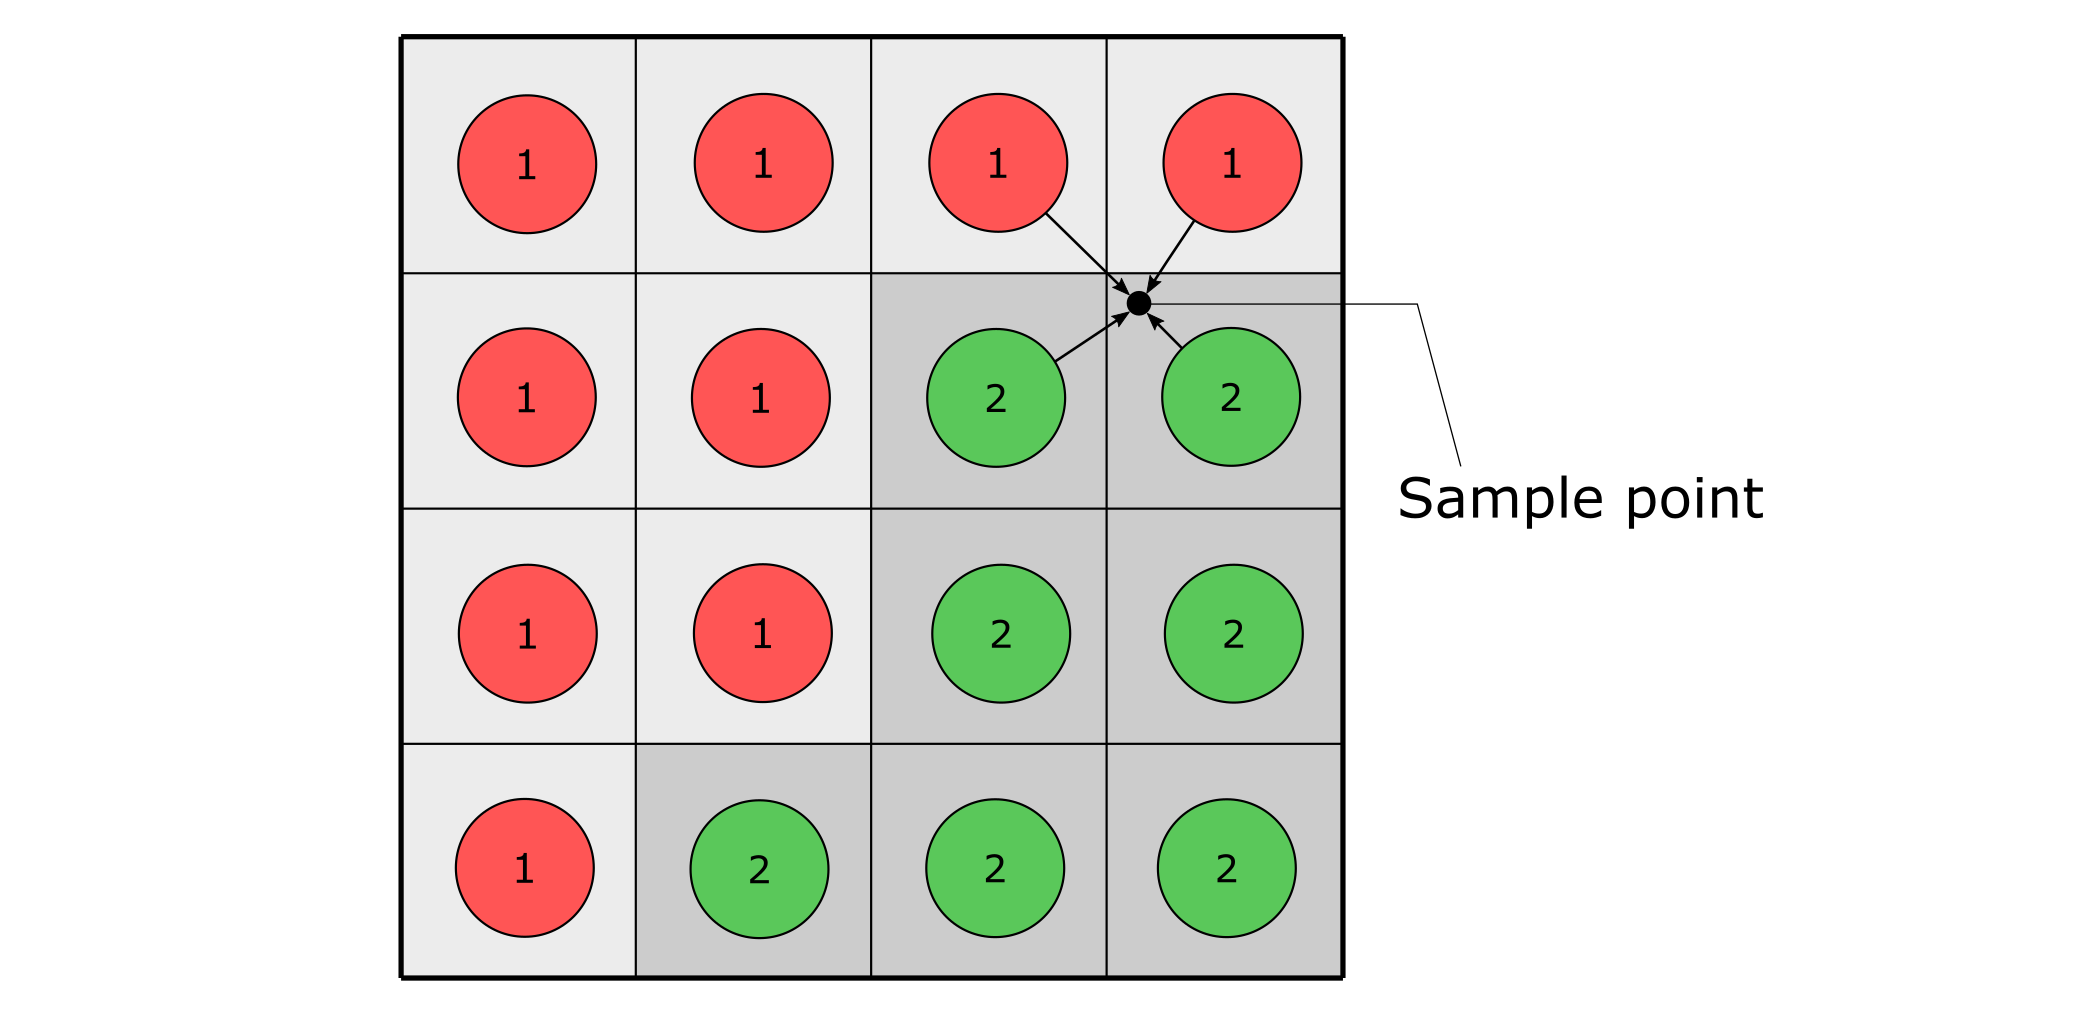
\includegraphics[width=\textwidth]{BilinearError}
\caption{
The texture unit uses blend masks from different Clusters during texture filtering.
The result of such filtering is a leaking of the material boundaries which leads to visual artifacts in the composition stage.
}
\label{Makeev-MaskFilteringError}
\end{figure}

\subsection{Spatial Clustering Encoding Representation}

At the preprocessing stage, we build a clustered representation using a single Color ID to define all the opaque materials and an ordered set of Material Masks to define all transparent materials.
As a result of preprocessing, we get a dataset which is used for the runtime composition and contains three different types of data.

\begin{itemize}  
\item \textbf{Cluster Indirection}.
An indirection texture that defines the current cluster ID for a specified texel.
The cluster ID is stored using an integer texture format and defines which set of materials should be used for a given texel.
Cluster Indirection is stored using a texture that has a lower resolution than a resolution of the source Material Masks.
Neighbor texels usually use the same set of materials and the set of used materials rarely changes which allows us to use a smaller resolution texture to store this data.
Since this texture contains the integer data, this texture cannot use any texture filtering.
Cluster Indirection is stored in the texture without mipmaps and fetched using a POINT texture filtering mode.
\item \textbf{Cluster Weights}.
The weight texture defines the blending weight for each material in a set of materials which a specified by the cluster ID.
We support up to five different material masks per pixel where the weights are stored using the BC3 texture format. 
Cluster Weights are stored using a texture that has the same resolution, as the input Material Masks, despite the set of used materials rarely vary, neighbor texels of a blend mask can differ significantly.
Cluster Weights can be correctly filtered inside the same material cluster.
Texture data is stored with mipmaps and fetched using a TRILINEAR or ANISOTROPIC texture filtering mode.
\item \textbf{Cluster Properties}.
Defines material surface properties such as albedo, roughness, metalness, etc. which are used for the final composition.
We decided to use a Structured Buffer to store the Cluster Properties.
Depending on the implementation, Cluster Properties can also be stored in the Constant Buffer.
\end{itemize}

At the composition stage, we obtain the cluster ID for each fragment which defines a set of used materials and the blending weights.
Then using the Cluster Properties, we obtain the surface properties for each material which are used in the current cluster.
Afterwards, we use the blend weights and the surface properties for the final composition of the surface properties for a given fragment. 
See Figure ~\ref{Makeev-ClusteredRepresentation} for more details.

\begin{figure}\centering
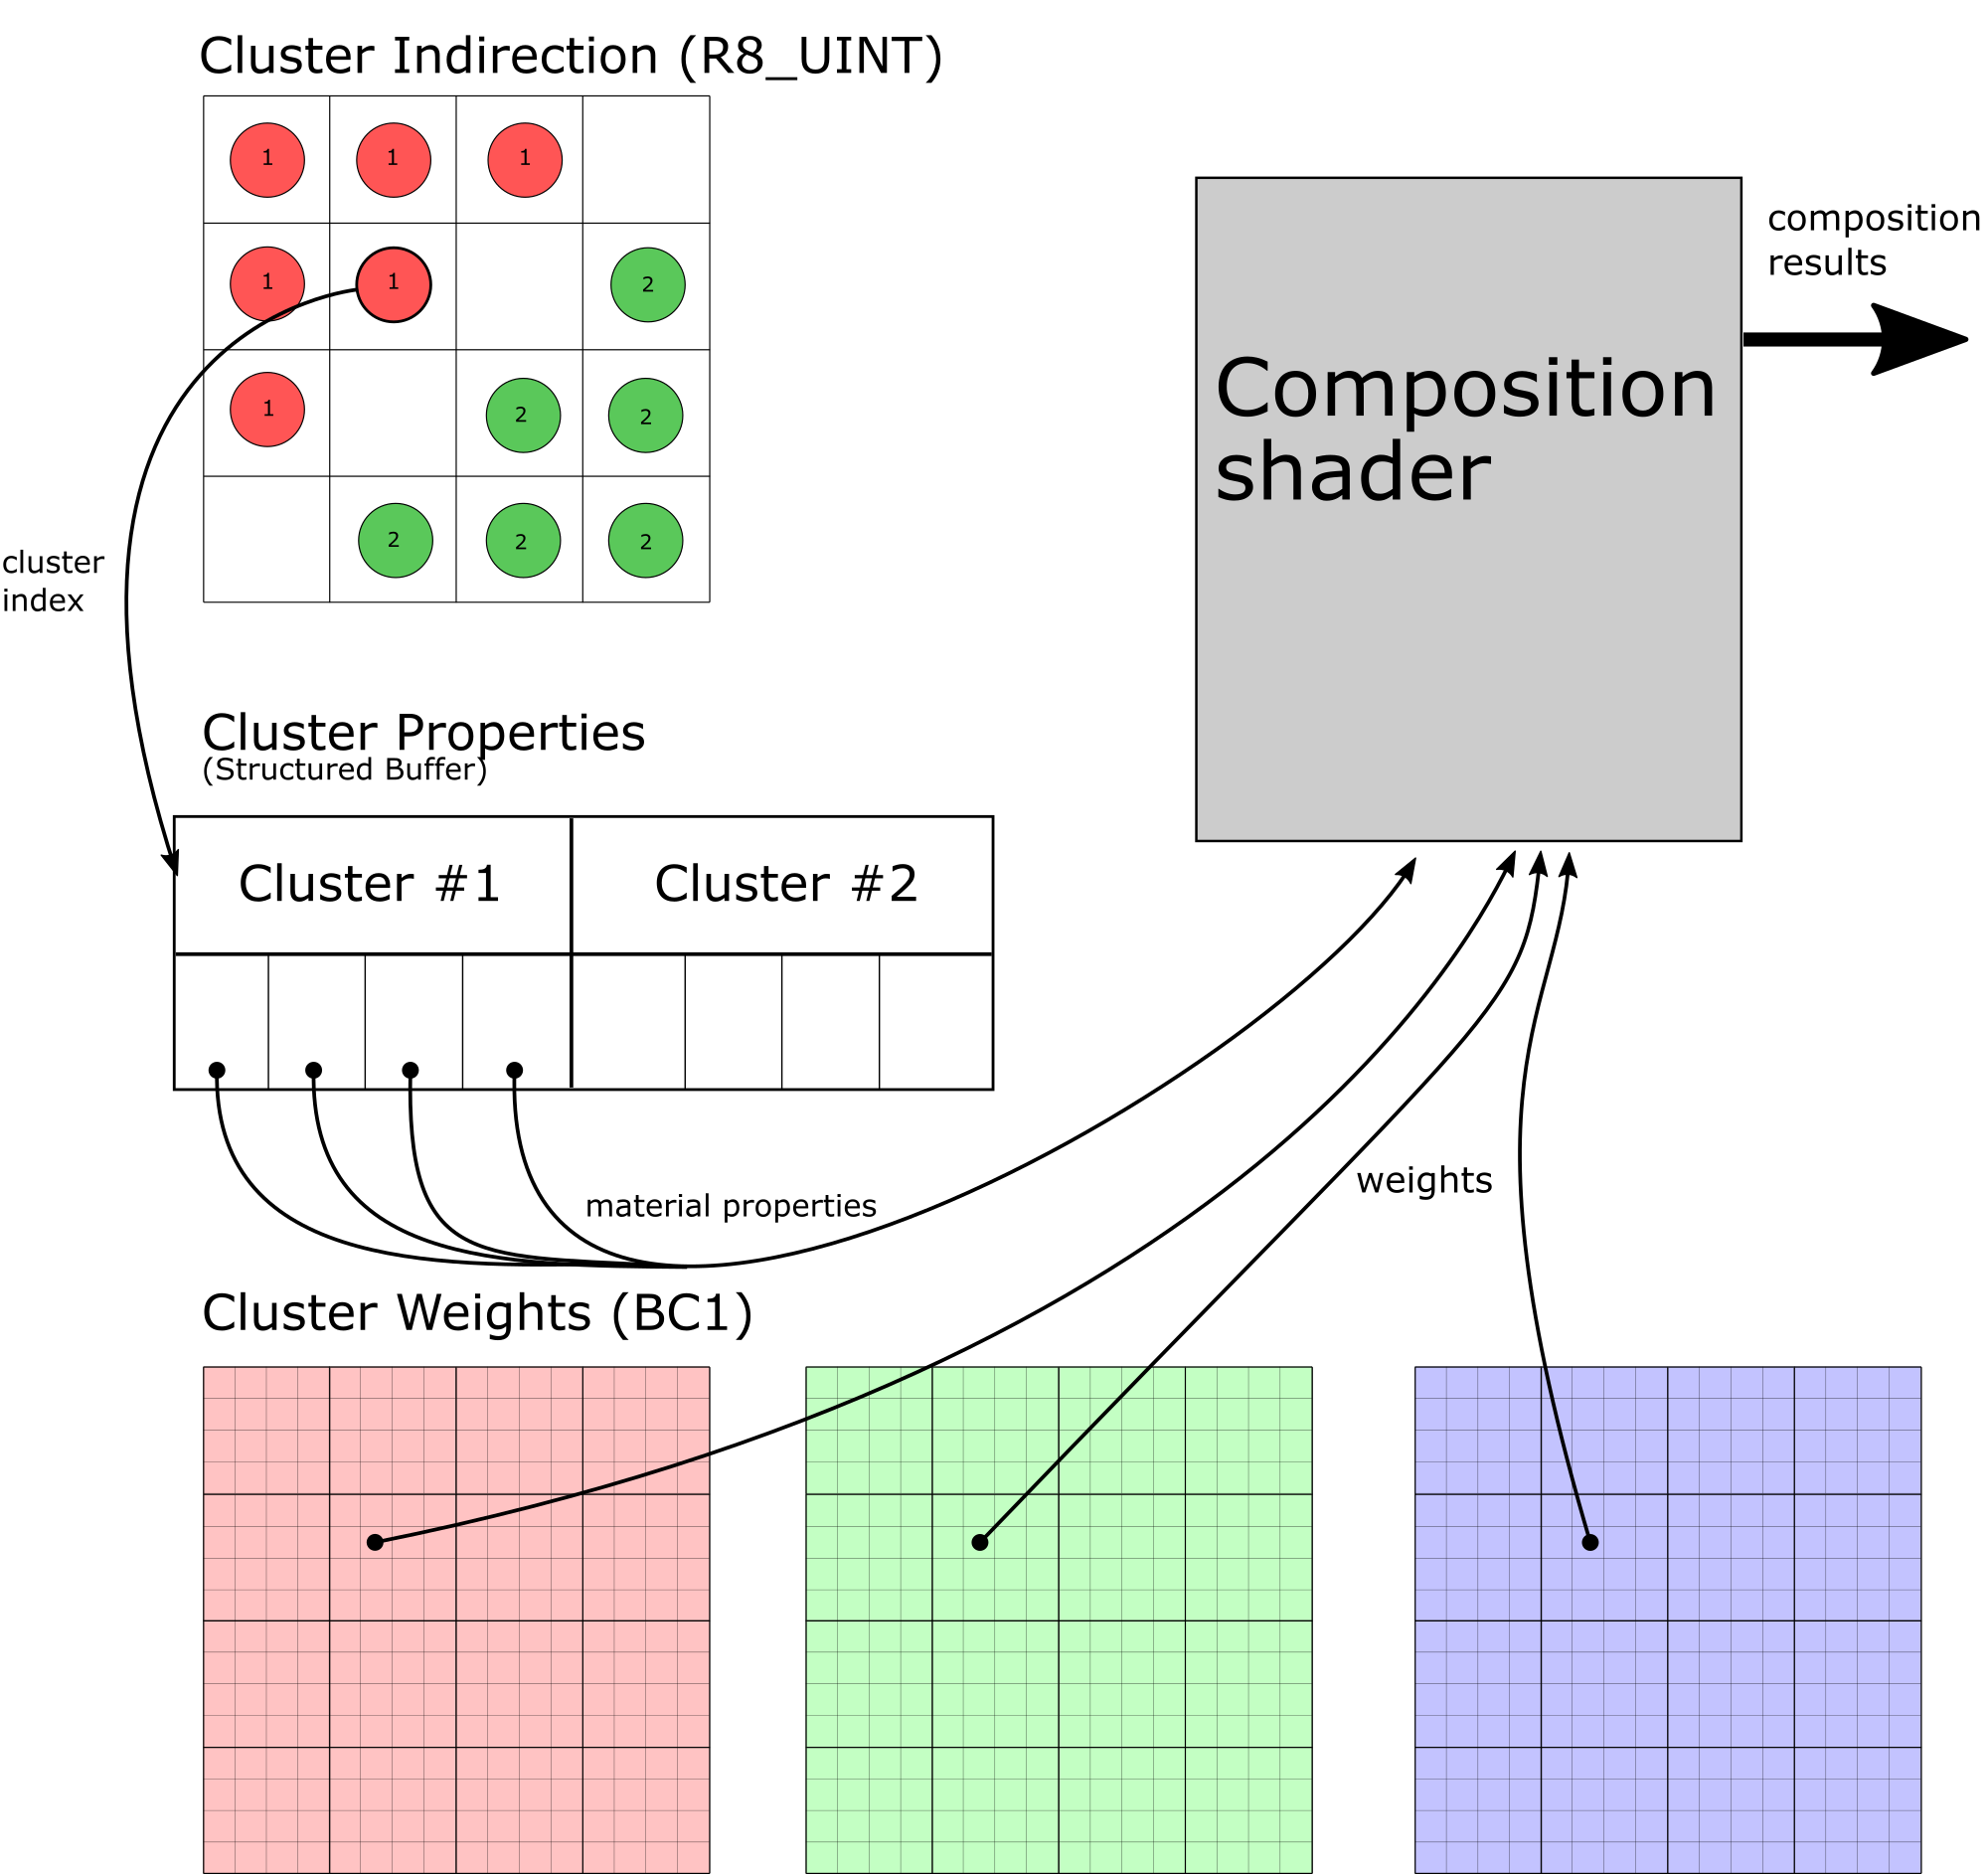
\includegraphics[width=\textwidth]{ClusteredRepresentation}
\caption{An example representation and usage of the encoded data.} \label{Makeev-ClusteredRepresentation}
\end{figure}

\subsection{Order-independent representation for blend masks}

For the final composition, we need to blend materials in the correct order, as defined in the input data.
The most common way of doing this is to perform alpha blending and composite the fragments in a back-to-front order using the following equation:

\[
C_{final} = C_{src} * \alpha + C_{dst} * (1 - \alpha)
\]

Then we repeat this operation for all the blend masks used for blending:

\[
C_{final} = \left[C_n \alpha _n +(1 - \alpha _n) \dots \left[ C_2 \alpha _2 + (1 - \alpha _2) \left[ C_1 \alpha _1 +(1 - \alpha _1)C_0 \right]\right]\right]
\]

This approach depends on the order of operations and instead of using alpha-blending we can rewrite the blending equation in weighted form:

\[
C_{final} = w_0 C_0 + w_1 C_1 + w_2 C_2 + \dots + w_n C_n 
\]

Where:

\[
w_{k} = (1 - \alpha _n) (1 - \alpha _{n-1}) \dots (1 - \alpha _{k+1}) \alpha_k
\]

Since the resulting weights are normalized, we know that the sum of all weights are always equal to one.
We can use this property to reconstruct one of the weights inside a composting pixel-shader instead of storing this weight in the texture channel:

\[
w_n = 1 - w_0 - w_1 - w_2 \dots - w_{n-1}
\]

For our implementation, we decided to use the order-independent weighted representation for the texture blend masks.
The order-independent representation allows us to swap the texture channels inside the cluster freely.
This property can be very useful for several further optimizations.

\section{Algorithm Implementation}

\subsection{Extract background materials}

First, we define an opaque material for each texel.
The opaque material is also used to determine which texels are inside the UV mapping and which ones are not.
Then we determine which texture resolution we should use for the latest supported mipmap level.
For each texel inside the mip-level, we generate a Color ID value from the original high-resolution Color ID texture.
To avoid situations where the resulting mipmap texel uses several different opaque materials, we forbid using different Colors IDs in the neighboring texels.
This natural limitation allows us to find potential clusterization issues at the very early stage of the art-pipeline and helps create Color ID maps which can be efficiently clustered.
This also allows us to skip the connectivity analysis for all the opaque materials since the different opaque materials never share the neighboring texels.

\subsection{Material layers}

At this step, we have the ordered set of texture blend masks called Material layers.
Each material layer defines the transparency of the blending for each texel.
We downsample each material layer using a MAX filter to the resolution corresponding the latest supported mipmap level.
If the resulting texel was marked as unused on the previous step, this texel is located outside of the valid UV mapping and will not be used in the composition. 

\subsection{Weighted sum representation}
\label{Makeev-WeightedSum}

At this step, we have several downsampled texture blend masks defined in the specified order used for the alpha blending.
We transform the texture blend masks to a normalized weighted form using Algorithm~\ref{Makeev-WeightSumAlgorithm}.
The normalized weighted representation also helps us to discard texels that are entirely covered by other materials and do not contribute to the final composition.

\LinesNumbered
\DontPrintSemicolon
\begin{algorithm}\label{Makeev-WeightSumAlgorithm}
\For{every \textbf{texel(X,Y)} in opaque layer}{
    \If{\textbf{texel(X,Y)} is empty in opaque layer}{
        skip texel \;
    }
    accum = 1.0 \;
    \For{every input texture blend mask}{
        alpha = \textbf{blend\_mask(X,Y)} \;
        \textbf{layer\_weight(X,Y)} = alpha * accum \;
        accum = accum * (1.0 - alpha) \;
    }
}
\caption{
Converting the texture blend mask to a normalized weighted form.
}
\end{algorithm}


\subsection{Undirected graph representation}

At this step, we move from a bitmap representation of input data to an undirected graph representation.
The advantage of a graph representation in comparison with a bitmap representation is that we can use graph theory for analyzing and building clusters with specific characteristics.
For each texel, we find all the texture blend masks that have contributed to a given texel, and assign a unique texel identifier that corresponds to the unique combination of blend masks used.
Then we find the connected area using an algorithm similar to a flood-fill algorithm and make a separate graph vertice from each unique combination.
The result produced by the algorithm shown in Figure~\ref{Makeev-GraphVertices}.
For each resulting graph vertice, we store an assigned identifier that encodes which blend masks were used to build this graph vertice.

\subsection{Texture filtering requirement analysis}

At this step, we build edges between graph vertices according to the following rule:
If two graph vertices have adjacent pixels that are used for texture filtering, these vertices are connected.

As a result, we built a connected undirected graph \emph{G = (V,E)} from the source bitmap data.
\emph{V} represents the area affected by the different combinations of input texture blend masks.
\emph{E} represents the texture filtering relationship between these areas as shown in Figure~\ref{Makeev-GraphLinks}.
The number of texels used for texture filtering determines the edge weight and will be used later for the graph partitioning.

\begin{figure}\centering
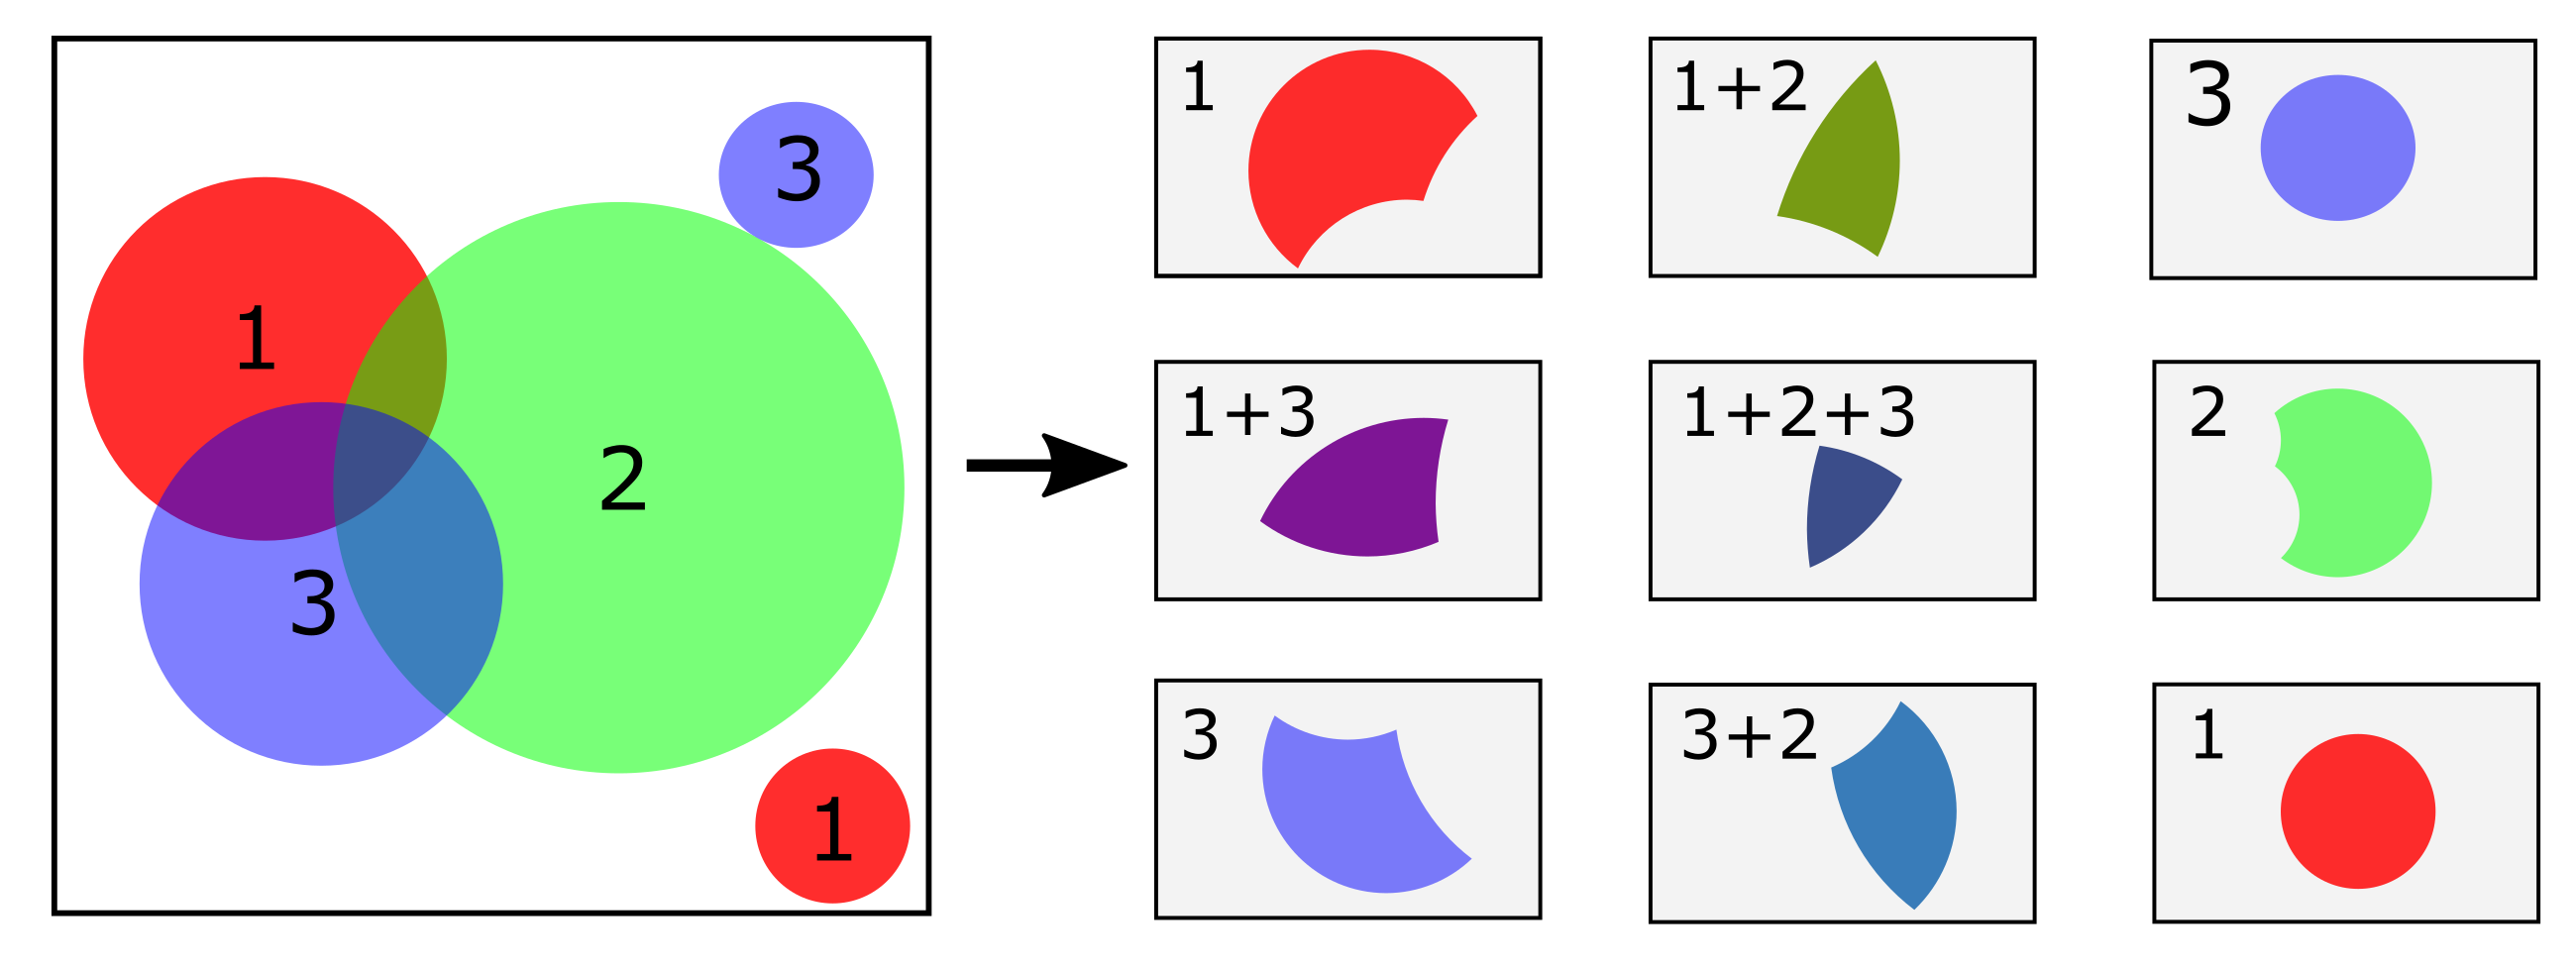
\includegraphics[width=\textwidth]{GraphNodes}
\caption{
Spliting bitmap data to the graph vertices.
Red, Green and Blue circles represent areas covered by the different texture blend masks.
}
\label{Makeev-GraphVertices}
\end{figure}


\begin{figure}\centering
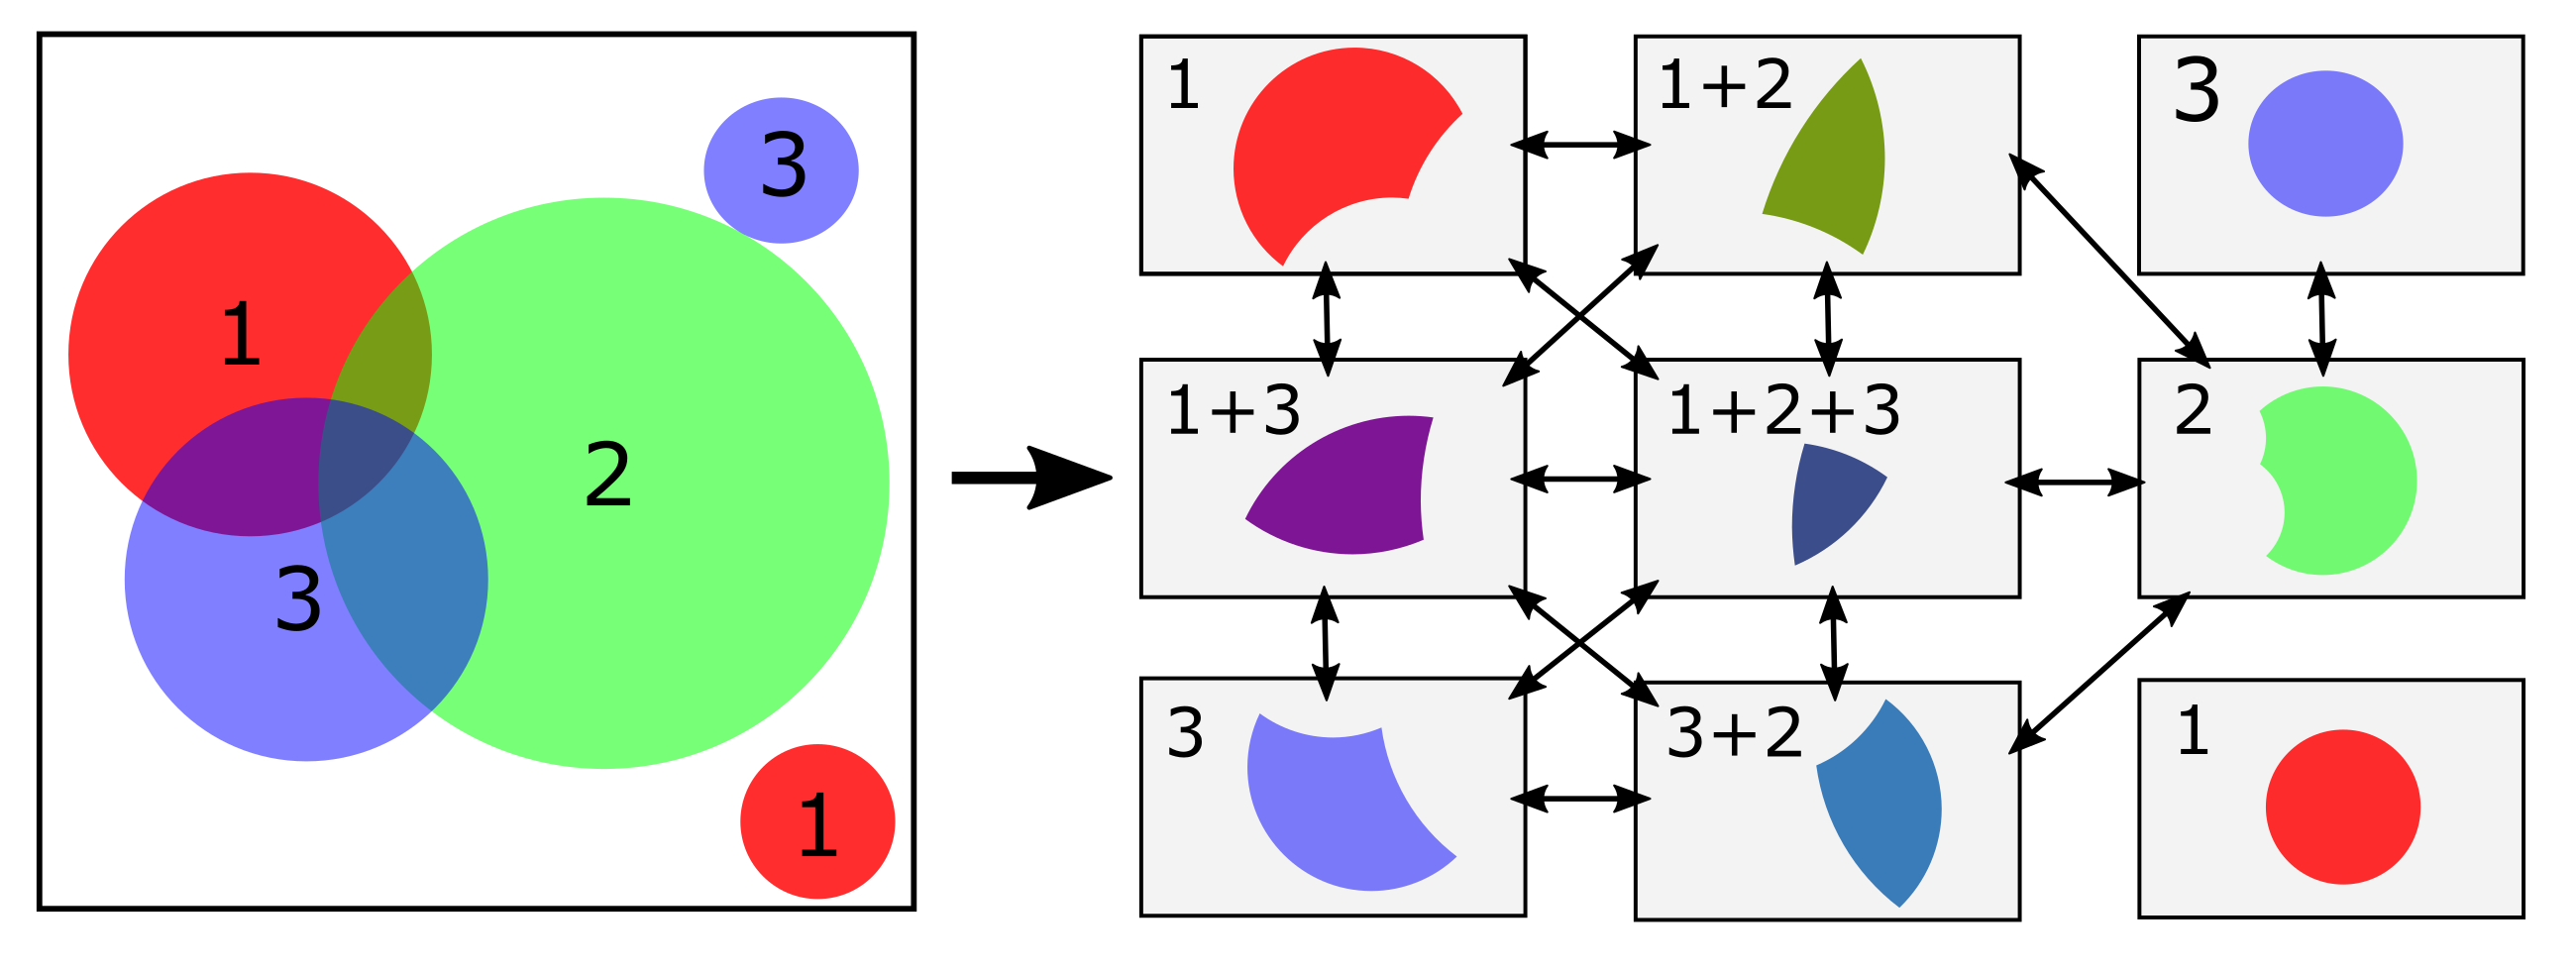
\includegraphics[width=\textwidth]{GraphLinks}
\caption{
Resulting undirected graph.
Arrows represent edges which indicate the texture filtering relationships between vertices.
}
\label{Makeev-GraphLinks}
\end{figure}


\subsection{Finding the number of connected components}

The resulting undirected graph usually has several connected components.
Our goal is to find the number of connected components and split the graph into several subgraphs between which no filtering is required (see Figure~\ref{Makeev-GraphComponents}).
Each subgraph is processed as an independent graph for the next algorithm steps.
If the resulting graph already fits our initial requirements and does not exceeding the maximum allowed number of materials, then the next step is redundant and can be skipped.
Otherwise, the next algorithm step splits the graph into several subgraphs with specific properties defined by our initial requirements.

\begin{figure}\centering
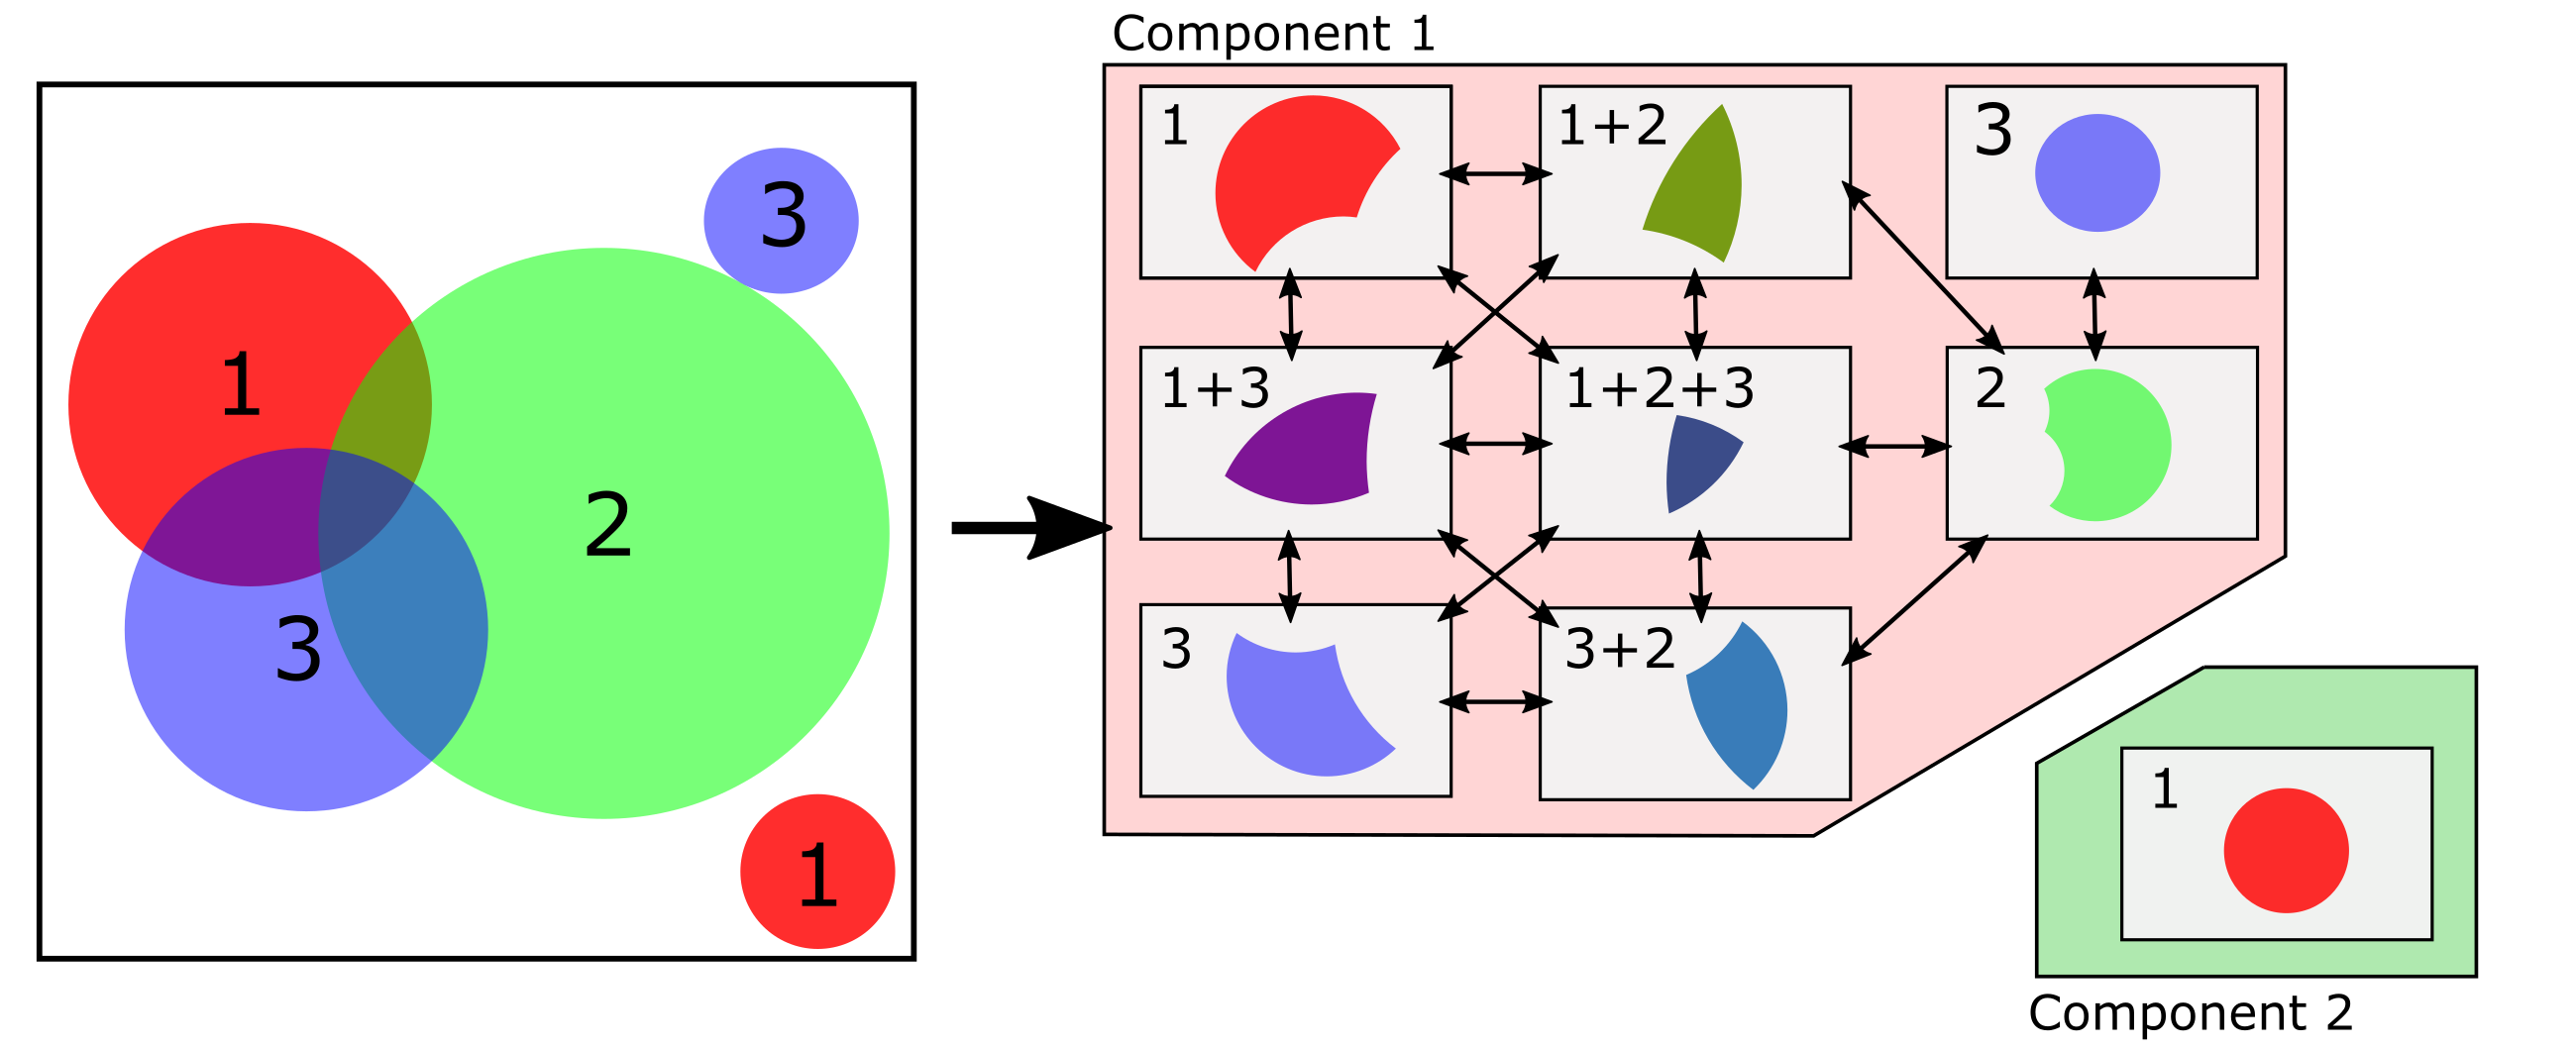
\includegraphics[width=\textwidth]{GraphComponents}
\caption{A resulting graph with two connected components.}
\label{Makeev-GraphComponents}
\end{figure}

\subsection{Solving the graph partitioning problem}
\label{Makeev-SolveGraphPartition}

At this step, we need to solve the graph partitioning problem and split a graph \emph{G = (V,E)}, where \emph{V} is the set of vertices and \emph{E} are edges, into smaller components with specific properties.
Typically, graph partition problems are NP-hard problems so we should use heuristics and approximations to solve the graph partition problem.
To find the optimal solution, we use an iterative greedy algorithm to find a set of edges with minimal weight to cut.
Our solution is inspired by the heuristic algorithm of graph partitioning proposed by Kernighan and Lin \cite{KernighanLin}.

Our goal is to divide the graph into subsets A and B where subset A satisfies initial requirements, and the sum of edge weights from A to B are minimized.
Since the weight of the edge is the number of pixels used for the texture filtering, by minimizing the sum of edge weights from A to B we reduce the resulting filtering error.
Our multi-pass algorithm maintains and improves a partition, using a greedy algorithm in each pass to pair up vertices of A with vertices of B, so that moving the paired vertices from one side of the partition to the other improves the partitioning.

Next, our algorithm chooses the best solution from all solutions that have been tried.
Thus our algorithm attempts to find the optimal subset A which has a minimum sum of edge weights to cut.
See Algorithm ~\ref{Makeev-GraphSplitAlgorithm} for implementation details.
To demonstrate one iteration step of the algorithm, see Figure~\ref{Makeev-GraphPartitioning}.

\SetKwFor{Loop}{begin\_loop}{}{end\_loop}
\LinesNumbered
\DontPrintSemicolon
\begin{algorithm}\label{Makeev-GraphSplitAlgorithm}
\ForEach{ \emph{source layers \underline{identifier} existing in the graph} G(V,E)}{
    \Begin(split graph into initial \textbf{subsets A} and \textbf{B}) {
    add all graph vertices with same \underline{identifier} to \textbf{subset A}\;
    add all other graph vertices into \textbf{subset B}\;
    }
    \Loop{}{
        calculate sum of edges weights between \textbf{subset A} and \textbf{B} and store as solution\;
        find a vertice inside a \textbf{subset B} that has the largest sum of edges crossing between subsets and can be moved to a \textbf{subset A} without violating our constraints\;
        \uIf{such vertice found}{
            move all vertices with same \underline{identifier} as a found vertice from the \textbf{subset B} to the \textbf{subset A}\;
        }
        \uElse{
          \textbf{break}\;
        }
    }
}
\Return solution with the minimal weight between subsets\;
\caption{Graph partitioning algorithm.}
\end{algorithm}


\begin{figure}\centering
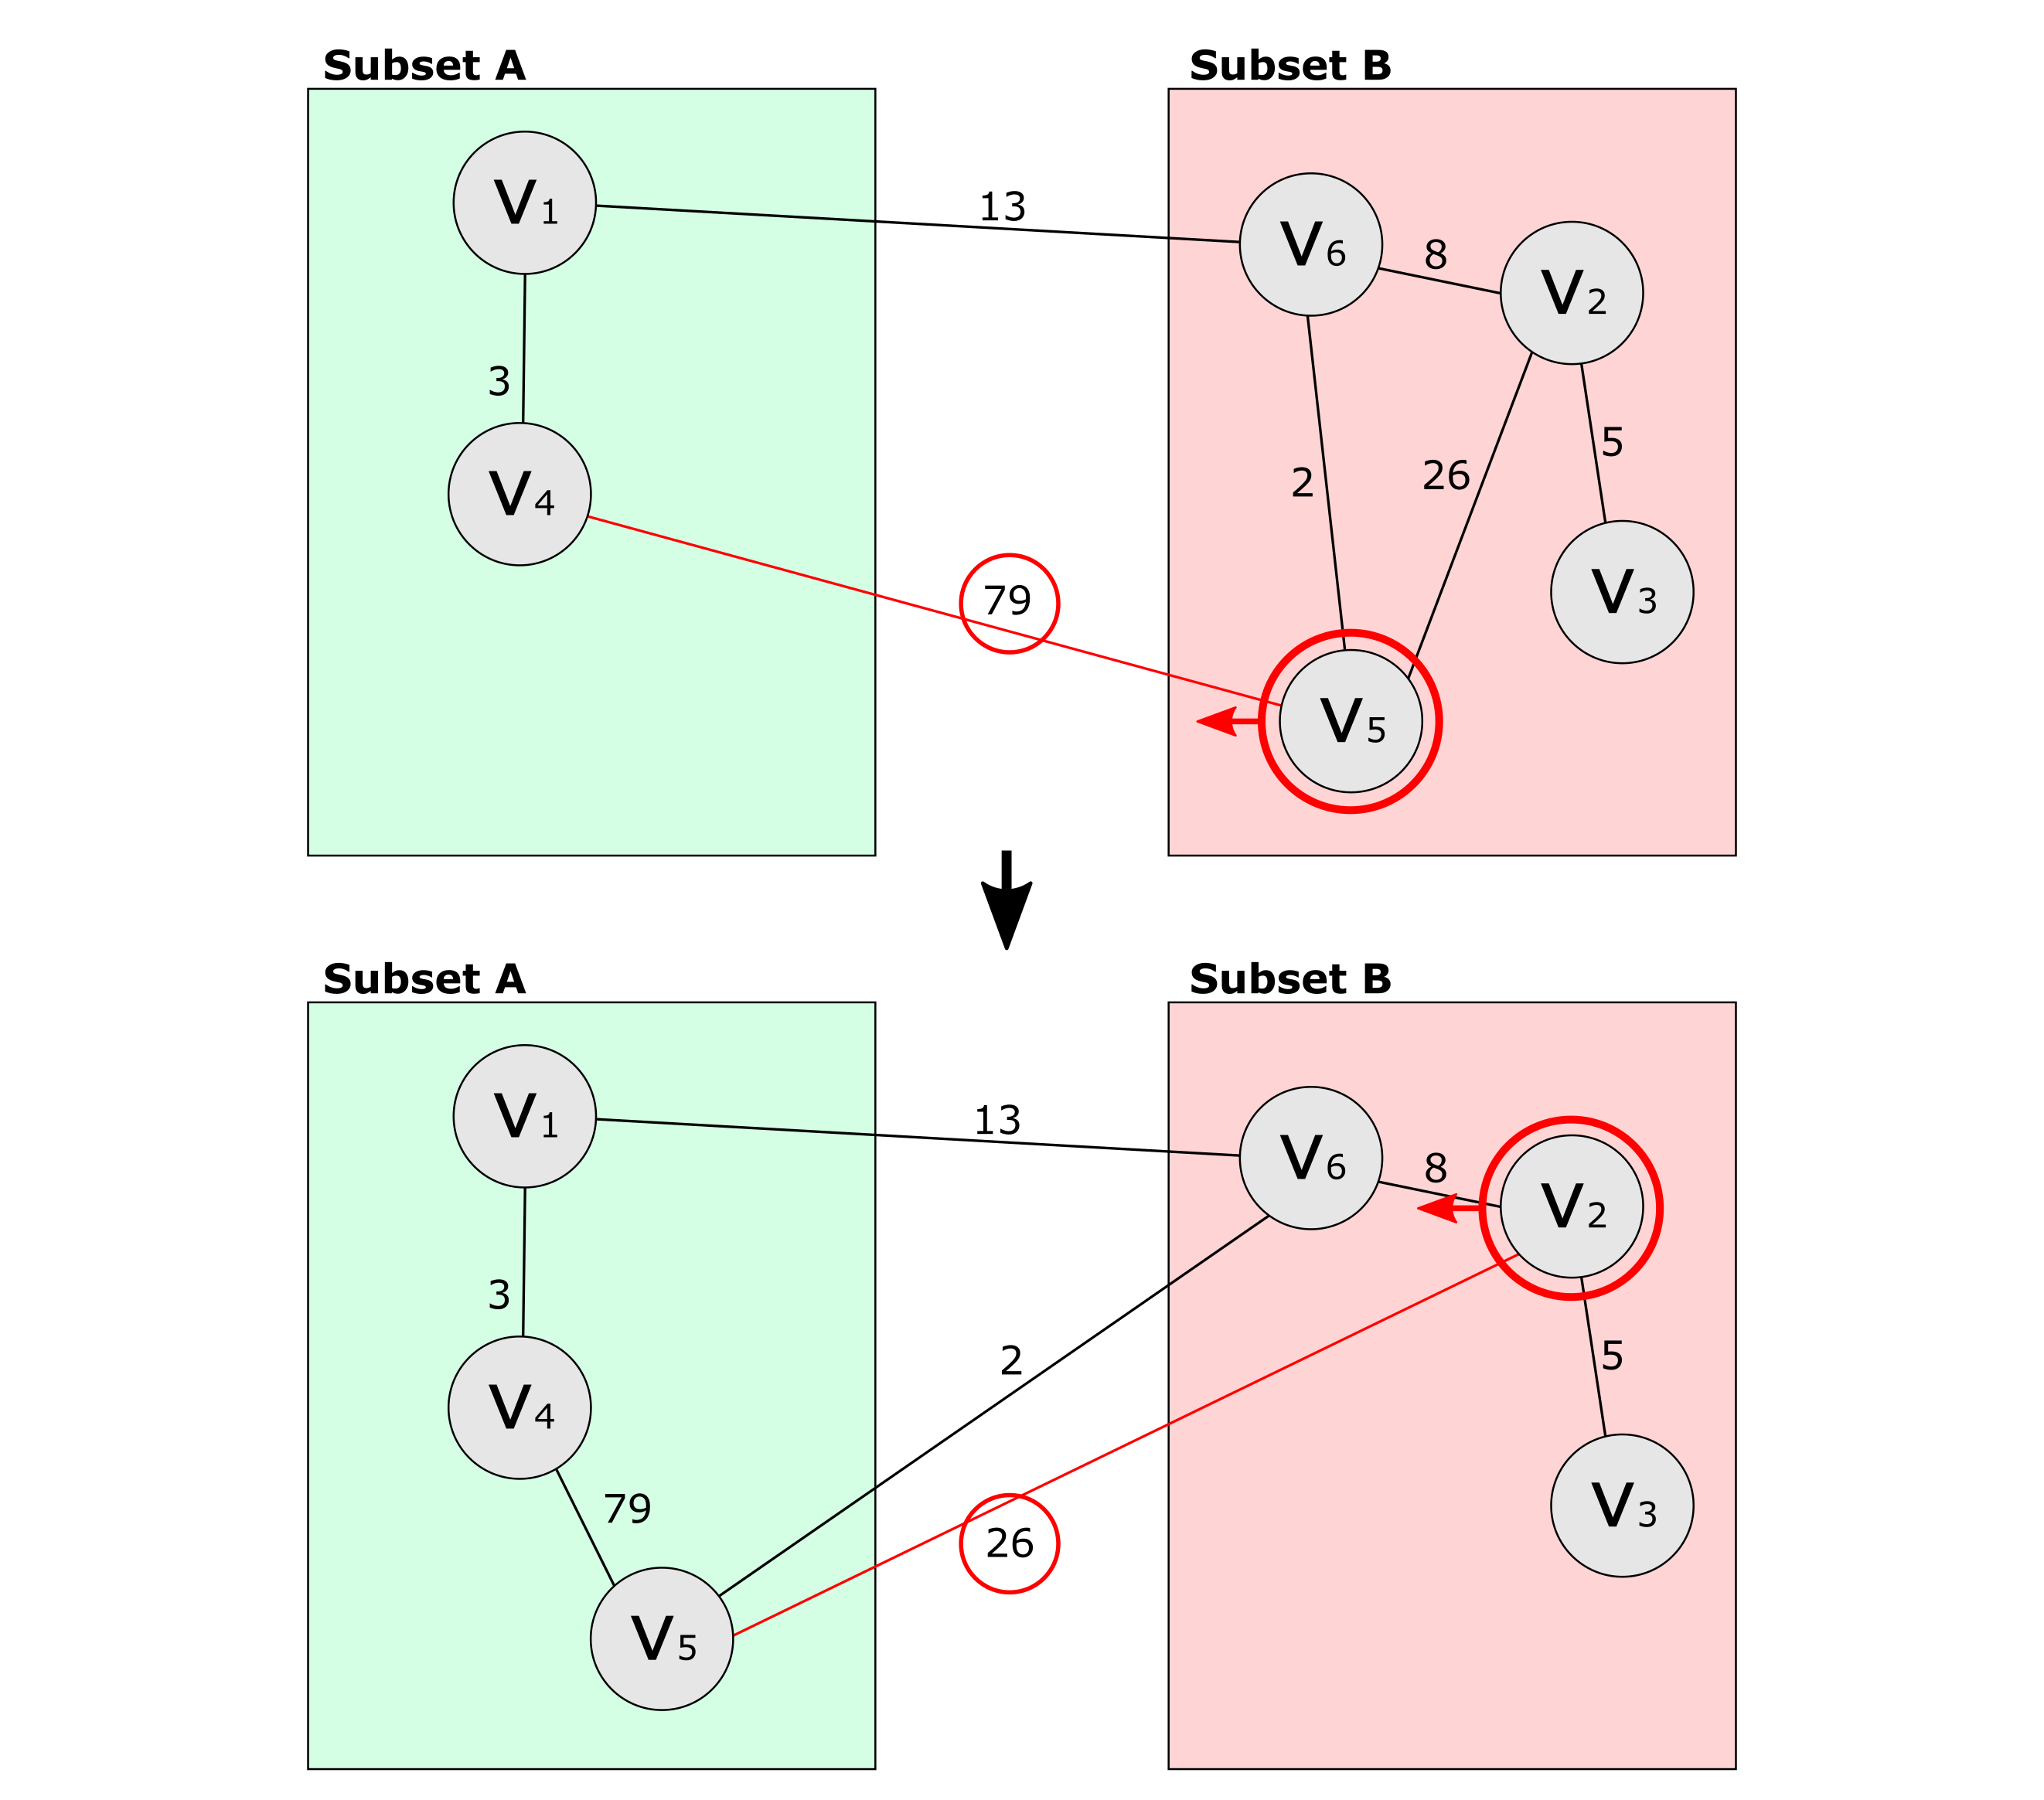
\includegraphics[width=\textwidth]{GraphSplit}
\caption{
One step of the graph partitioning algorithm.
The veritice V\textsubscript{5} moved from subset B into subset A.
} \label{Makeev-GraphPartitioning}
\end{figure}

\subsection{Generating the final data}

At the final step, we have a set of undirected graphs, where each graph fits our initial requirements.
In practice, many resulting graphs use fewer materials than the maximum allowable number.
To reduce the resulting number of clusters, we combine such graphs into larger ones as long as the merged results satisfy the initial requirements.


Next, we a build normalized weighted representation as described in Section~\ref{Makeev-WeightedSum}, but this time for full-resolution texture data.
For each resulting graph, we copy all texels used by the graph vertices from the weight textures into separate channels of the Cluster Weights texture.
Then we store the used graph index into a Cluster Indirection texture using the R8{\_}UINT format.
Next, for the Cluster Weights, we generate a partial mipmap chain which is limited by the number of supported mipmaps and then compress the resulting texture using the BC1 or BC3 texture format.
See Figure ~\ref{Makeev-FinalData} for the example set of resulting textures.

\begin{figure}\centering
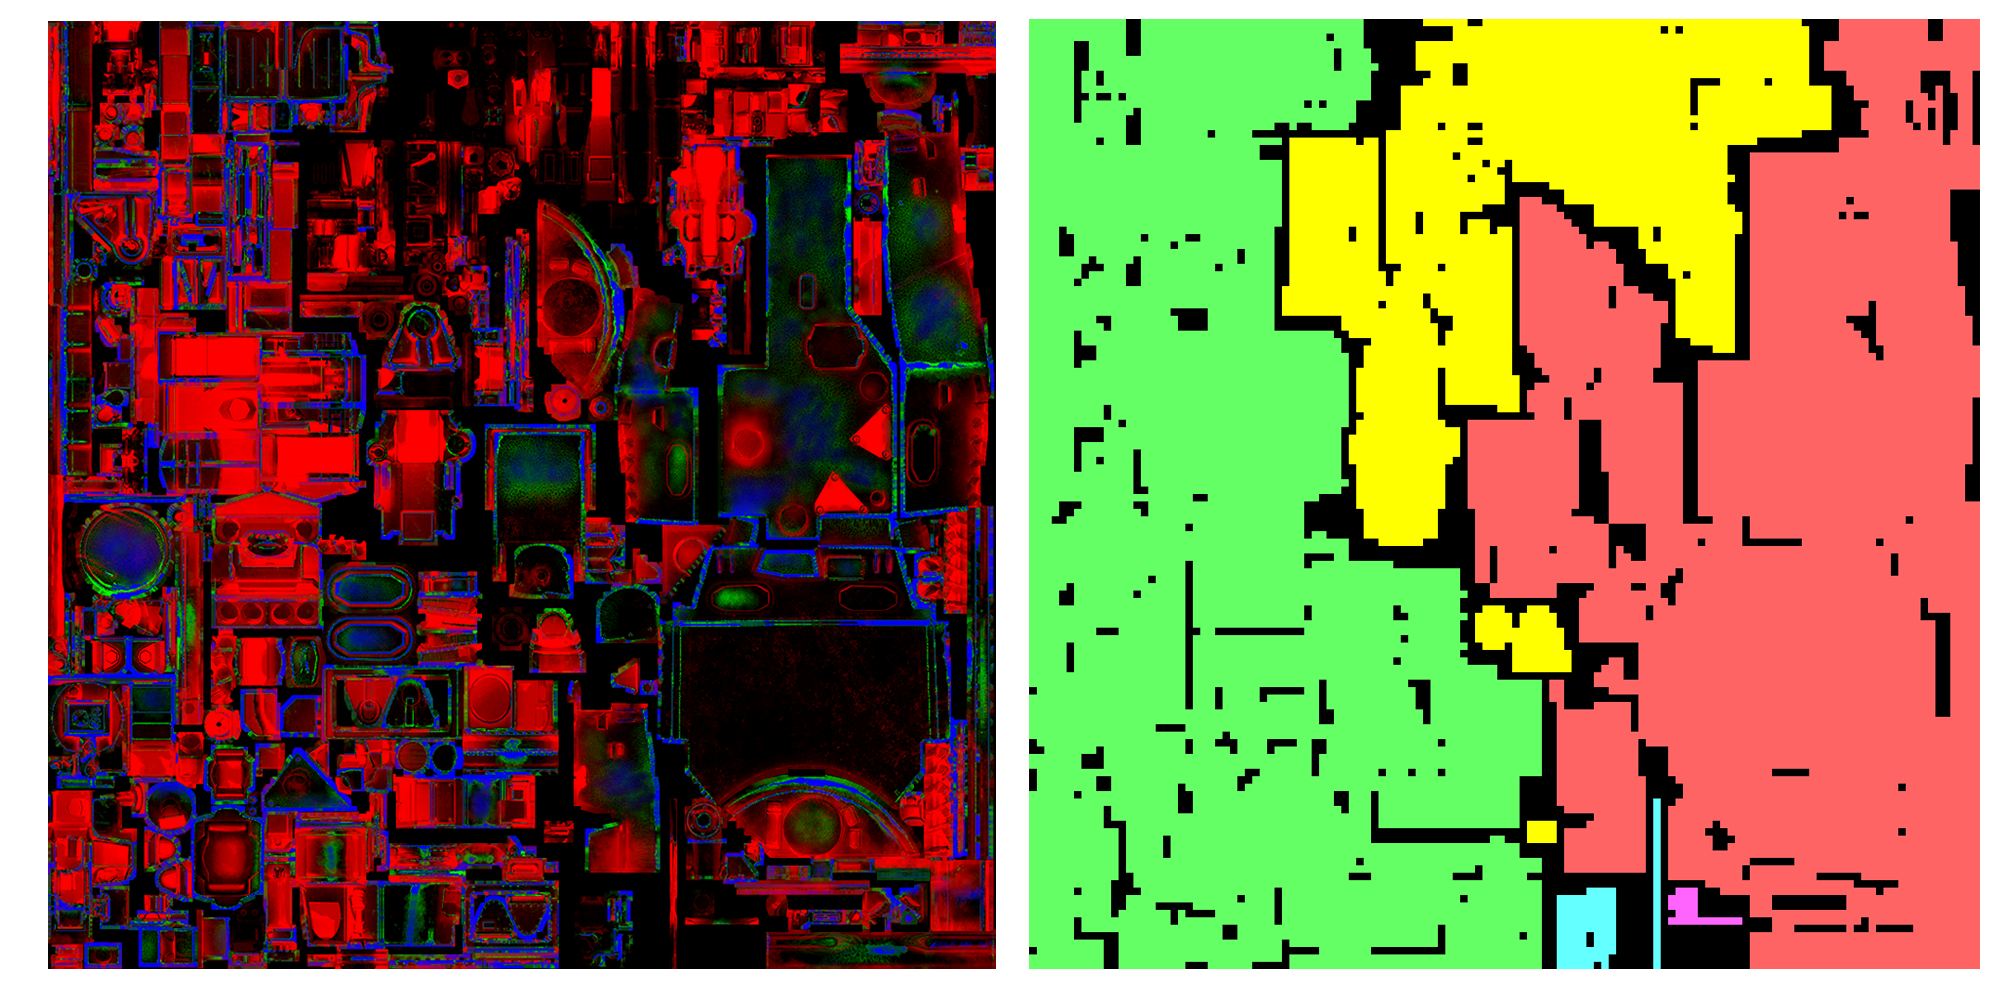
\includegraphics[width=\textwidth]{FinalData}
\caption{Final data generated by our implementation. Cluster weight texture (left) and Indirection texture (right). Indirection texture is colorized and upscaled by 8 times for demonstration purposes. Image courtesy of Mail.Ru Group.} 
\label{Makeev-FinalData}
\end{figure}

\subsection{Runtime Composition}

For the final composition of the material at runtime, we use the following approach:\par

\begin{itemize}  
\item Fetch the encoded cluster ID from the indirection texture.
\item Fetch material blend weights from the weight texture.
\item Read the surface properties stored in the Structured Buffer using the fetched cluster ID.
\item Make the final composition using the obtained surface parameters and material blend weights. See Listing~\ref{Makeev-ClusterDecode} for an example of a basic compositing shader.
\end{itemize}

Since we use a normalized weighted representation for storing the blend weights, we can change the blend weight of any individual material layer and renormalize the total sum of the weights.
This allows us to change the transparency of individual layers at runtime.

Textures used for the composition usually have insufficient resolution.
To increase the final resolution of the composition, we use detail textures stored in the texture arrays as described in \cite{BFPhotogrammetry}.
To generate UV-set for detail textures, we multiply original UV-set by tiling factor.
Tiling factor for detailed UV-set can be specified per material.
We use two sets of texture arrays: First for the surface parameters (albedo, roughness, metallic) and the second for the normal maps.
Each material used in the composition can use an arbitrary detail map for the surface properties and an arbitrary detail map for the surface normals.
See Figure ~\ref{Makeev-SurfaceDetails} for examples of the composition with and without detail textures. 

\begin{figure}\centering
\includegraphics[width=\textwidth]{DetailMap}
\caption{Rendering using detail maps (left) and without detail maps (right). Image courtesy of Mail.Ru Group.} \label{Makeev-SurfaceDetails}
\end{figure}

For the normal maps blending, we use a weighted blending of partial derivatives as described in "Blending in Detail" \cite{NormalsBlending}.
Additionally, we can blend only two detail maps with the highest contribution weights at a medium distance and completely disable detail maps at a long distance to improve the composition performance.

\subsection{Source code}

For demonstration purposes, we implemented our method using C\# for preprocessing and the Unity game engine by Unity Technologies for the runtime materials composition.
Full source code can be found in the supplemental materials of this book.


Source code is also available at \underline{\smash{https://github.com/SergeyMakeev/GpuZen2}}

\section{Results}

We used the approach described in this article for rendering the armored vehicles in the "Armored Warfare" game.
In our game, users can customize coloring and materials used for rendering the armored vehicles.
The presented technique allows minimizing the number of textures stored on disk while supporting high-quality textures and allowing the customization of the visual appearance.
You can see some results of using our technique in Figure~\ref{Makeev-AWRes}.
We compared the number of instructions resulting for our technique and number of instructions resulting for Unreal Engine 4 material layering technique, see Table~\ref{Makeev-PerfTable}.
Table~\ref{Makeev-ResultsTable} shows build times and the number of resulting materials clusters made for the armored vehicle.

\begin {table}
\begin{center}
    \begin{tabularx}{1\textwidth}{ | p{3.5cm} | X | X | X | X | X | }
    \hline
    Technique & Per-pixel number of layers & Total number of layers & Per-pixel number of detail-textures & ALU & TEX \\ \hline
    \textbf{Unreal Engine 4} - MatLayerBlendSimple & 4 & 4 & 4 & 82 & 14 \\ \hline
    \textbf{Unreal Engine 4} - Custom material & 3 & 3 & 0 & 23 & 2 \\ \hline
    \textbf{Spatial Clustering Encoding} - High & 5 & 9+ & 5 & 140 & 13 \\ \hline
    \textbf{Spatial Clustering Encoding} - Standard & 4 & 9+ & 4 & 104 & 11 \\ \hline
    \textbf{Spatial Clustering Encoding} - Fast & 4 & 9+ & 1 & 42 & 4 \\ \hline
    \textbf{Spatial Clustering Encoding} - Fastest & 3 & 9+ & 0 & 26 & 3 \\ \hline
    \end{tabularx}
\end{center}
\vspace*{-5mm}
\caption {Number of instructions resulting for different layered material techniques.} \label{Makeev-PerfTable}
\end {table}


\begin {table}
\begin{center}
    \begin{tabularx}{\textwidth}{ | X | X | X | X | X | X | X |}
    \hline
    Asset & Input materials count & Build time & Mips count & Graph vertices count & Clusters count & Memory used for cluster parameters \\ \hline
    \textbf{Turret} & 9 & 1.9 sec & 3 & 1791 & 5 & 560 bytes \\ \hline
    \textbf{Hull} & 7 & 1.4 sec & 3 & 3937 & 3 & 336 bytes \\ \hline
    \textbf{Cannon} & 7 & 0.5 sec & 3 & 262 & 4 & 448 bytes \\ \hline
    \textbf{Wheels} & 6 & 0.9 sec & 3 & 1422 & 3 & 336 bytes \\ \hline
    \textbf{Tracks} & 5 & 0.2 sec & 3 & 268 & 1 & 112 bytes \\ \hline
    \end{tabularx}
\end{center}
\vspace*{-5mm}
\caption {Build time and resulting cluster statistics for example asset.} \label{Makeev-ResultsTable}
\end {table}

\section{Conclusion and Future Work}

The method described in this chapter helps to store efficiently and use more texture blend masks than would be allowed by existing methods with some natural limitations.
Also, the proposed method supports real-time material recomposition using the proposed data representation. 
For the most effective use of our method, it is necessary to take into account the texture space connectivity of the different texture blend masks at the earliest stages ofthe  art-pipeline.
At the same time, the proposed method is suitable for any existing art assets without additional preparation with some tolerable texture filtering errors.
We are continue to develop and refine of the proposed technique.
Here are some areas for further development:

\begin{itemize}  
\item Nonlinear blending for the material composition as proposed in \cite{BlendMaps}.
\item Reducing the texture filtering errors when dividing clusters.
Since the texture blend masks are order independent, we can swap the texture channels inside the cluster.
Using the least squares minimization technique along the "seams" boundary as proposed in \cite{IwanickiLightmaps}, we can reduce the texture filtering error almost to zero.
\item Composition after evaluating BRDF instead of the surface properties composition.
Using this approach we can create accurate multi-layered materials with multiple specular lobes.
\item Using the vertex color as a blend weight modifier for local dynamic material recomposition (dynamic dirt, scratches, etc.).
\end{itemize}

\section{Acknowledgements}

First, I would like to thank Vladimir Egorov, my friend and colleague, for his suggestions and early feedback on this article.
Peter Sikachev, Vadim Slyusarev, Bonifacio Costiniano and Alexandre Chekroun for their feedback on this article.
In addition, I would like to thank all Allods Team members as well.

\definecolor{Makeev-CommentsGreenColor}{rgb}{0.0, 0.5, 0.0}
\lstset{language=C,commentstyle=\color{Makeev-CommentsGreenColor}\ttfamily}
\begin{lstlisting}[float=b,caption={An example of cluster decoding.},label=Makeev-ClusterDecode,numbers=left]
struct SurfaceParameters
{
 float3 albedo;
};
struct ClusterParameters
{
 SurfaceParameters layer0;
 SurfaceParameters layer1;
 SurfaceParameters layer2;
 SurfaceParameters layer3;
};
// Weights texture
Texture2D cWeights;
// Indirection texture
Texture2D cIndirection;
// Material parameters (stored per cluster)
StructuredBuffer<ClusterParameters> clusterParameters;

float4 DecodeAndComposition( float2 uv ) : SV_Target0
{
   float4 weights;
   // Fetch weights
   weights.xyz = cWeights.Sample(samplerTrilinear, uv).rgb;

   // Reconstruct weight
   weights.w = 1.0 - weights.x - weights.y - weights.z;

   // Fetch index
   uint clusterIndex = cIndirection.Sample(samplerPoint, uv).r;

   // Get material params 
   ClusterParameters params = clusterParameters[clusterIndex];

   // Use the material parameters and weights
   //                       for a final composition
   float3 albedo = params.layer0.albedo * weights.x +
                   params.layer1.albedo * weights.y +
                   params.layer2.albedo * weights.z +
                   params.layer3.albedo * weights.w;

   return float4(albedo, 1.0);
}
\end{lstlisting}

\begin{figure}\centering
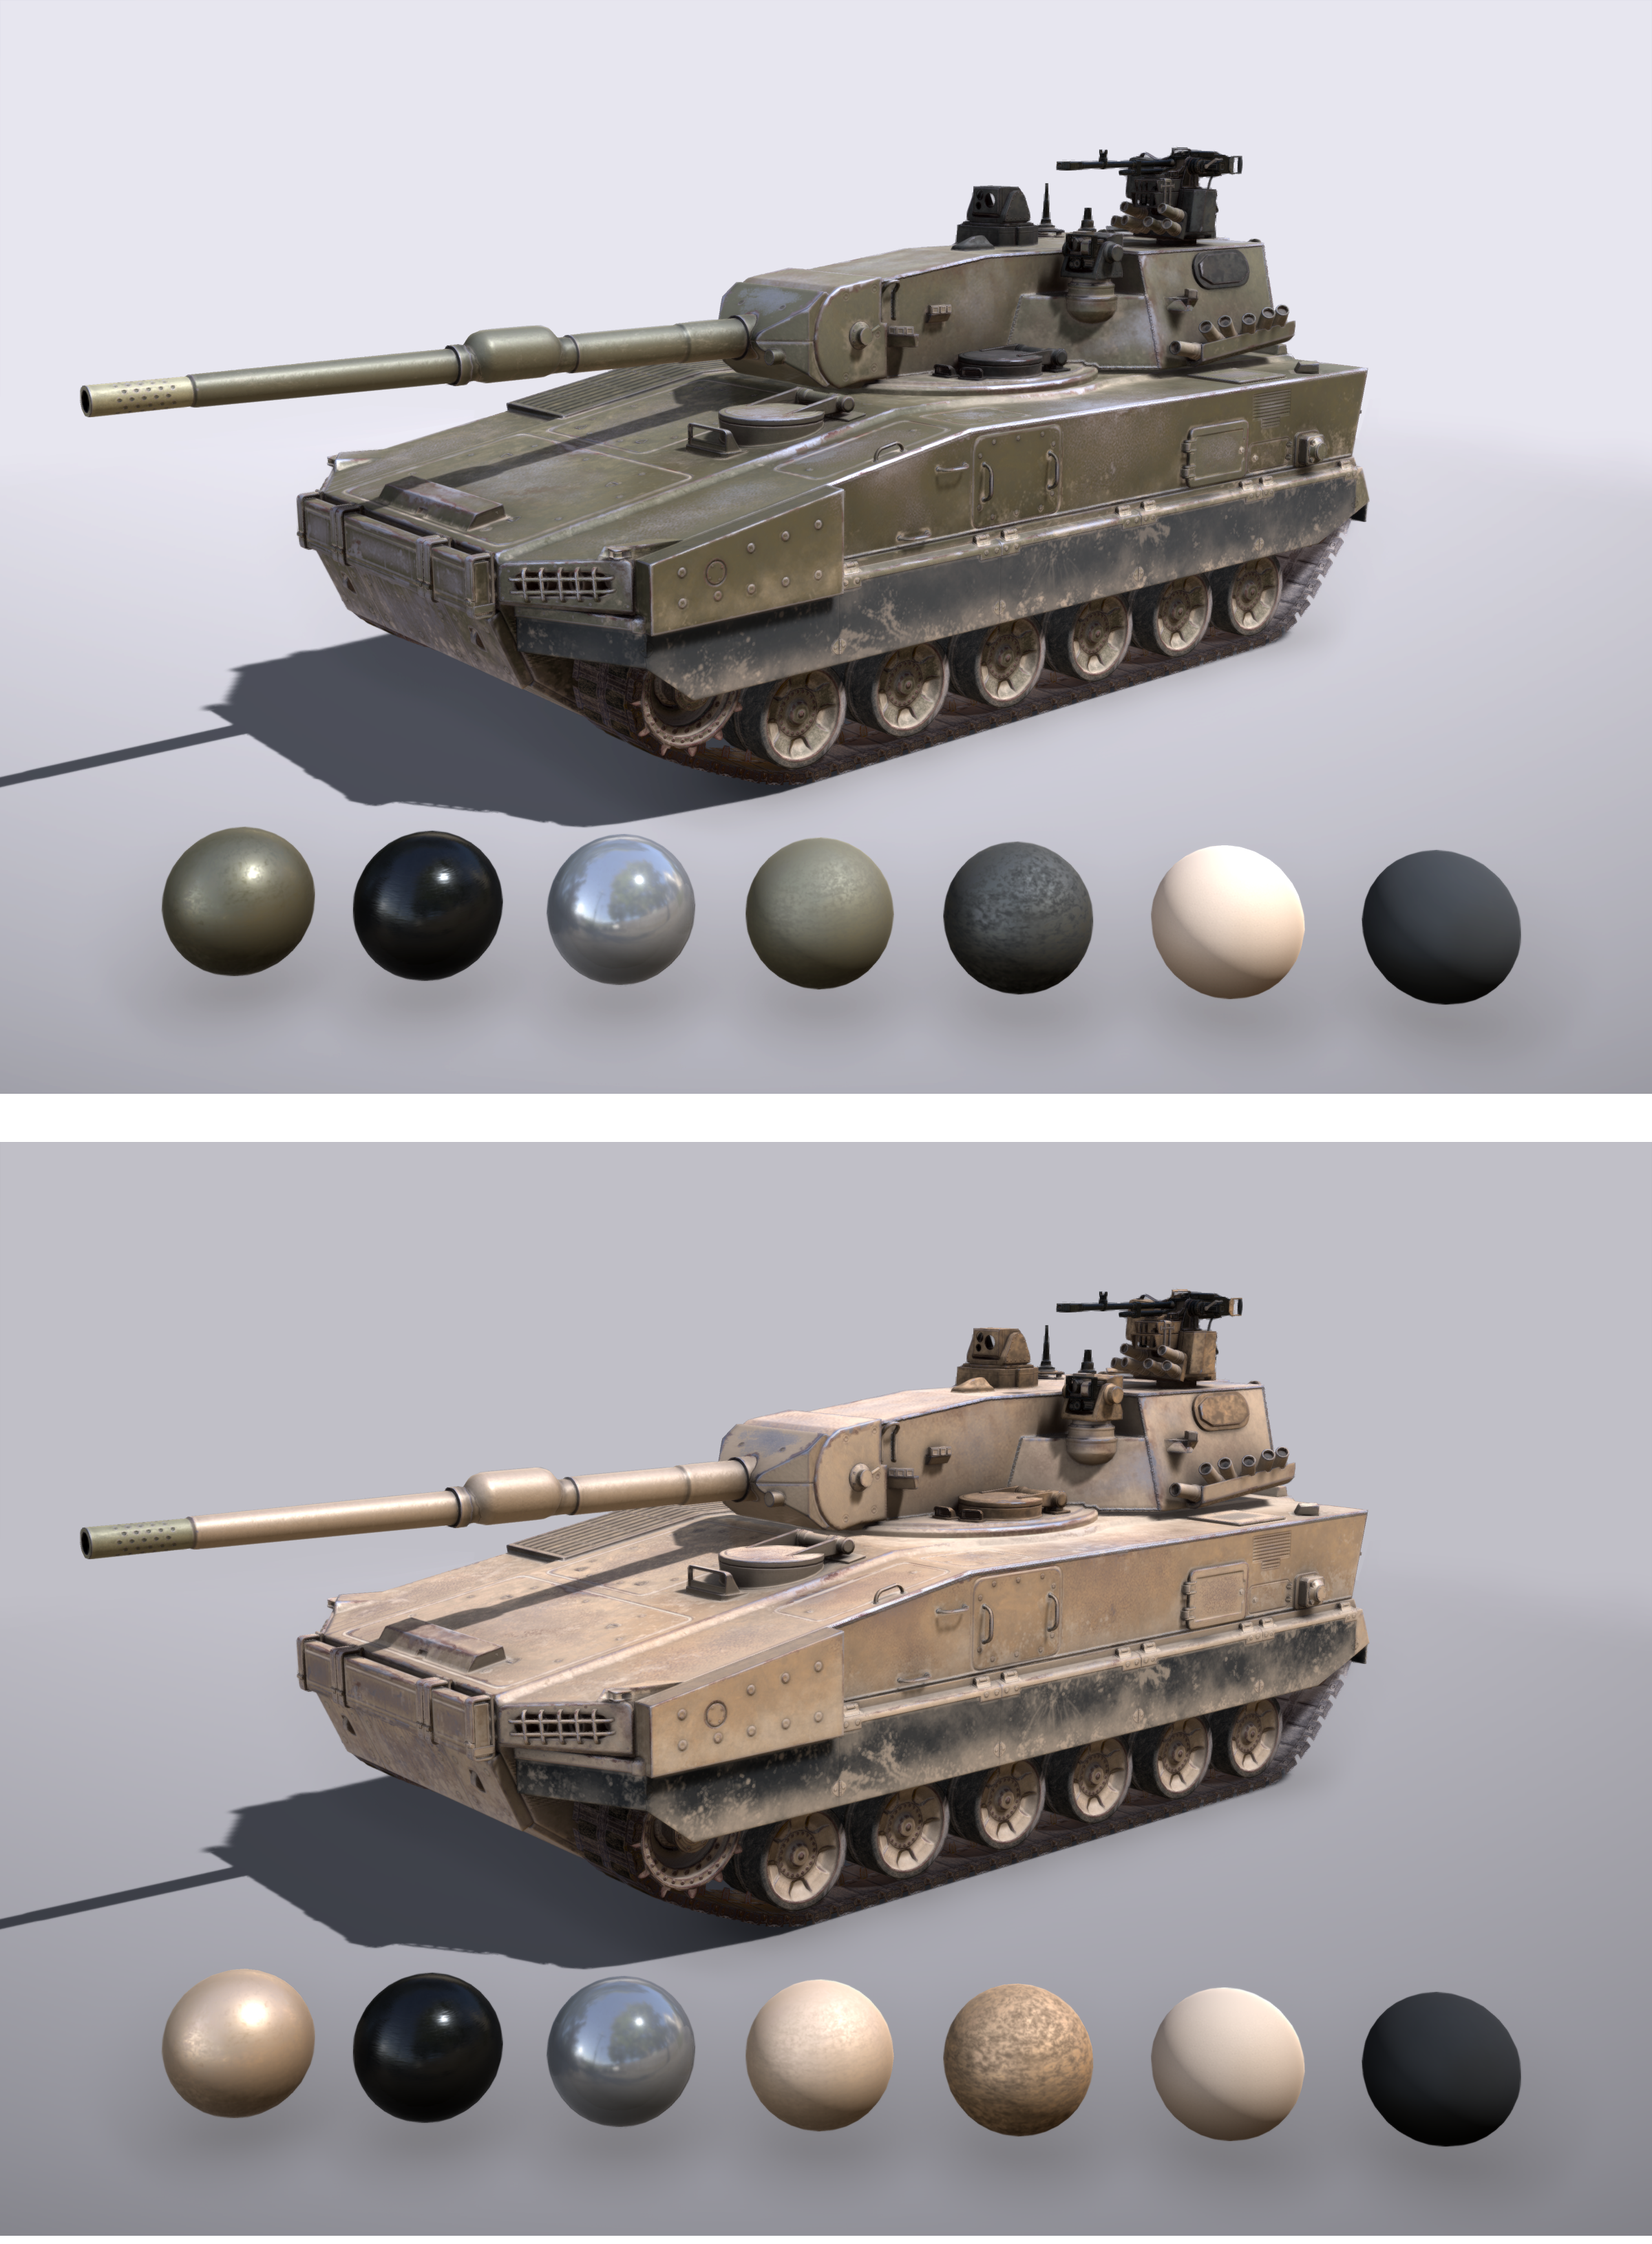
\includegraphics[width=\textwidth]{ArmoredWarfareResCombined}
\caption{
An example of composited material and some material templates used in composition (Top) and the same composited material with different material templates applied (Bottom).
Image courtesy of Mail.Ru Group.
} \label{Makeev-AWRes}
\end{figure}



\FloatBarrier

\bibliographystyle{akpbib}
\bibliography{Makeev}

%---END AUTHOR EDIT---

%*******************************************************************************
% Back Matter
%   Back matter begins with the bibliography.  We strongly recommend using a
%   .bib file.  You are welcome to use another bibliography style instead of our
%   in-house style.  For final production, the generated file can be renamed to
%   bibliography.tex. This file can be edited as needed, usually to fix breaks.
%
%   The index follows.  The index is generated using \makeindex (see above).
%   Use \printindex to display the index.
%
%*******************************************************************************
\backmatter
 \renewcommand{\chaptermark}[1]{\markboth{#1}{#1}}

\raggedright
\printindex

\end{document}
